\documentclass[11pt,a4paper]{article}
\usepackage[margin=23mm]{geometry}
\usepackage[T1]{fontenc}
\usepackage[utf8]{inputenc}
\usepackage{lmodern,microtype}
\usepackage{amsmath,amssymb,bm}
\usepackage[table]{xcolor}
\usepackage{booktabs,longtable,tabularx,array}
\usepackage{enumitem}
\usepackage[most]{tcolorbox}
\usepackage{tikz}
\usetikzlibrary{arrows.meta,positioning}
\usepackage{capt-of}
\tikzset{
  flow/.style={draw=ink,thick,rounded corners=2pt,fill=paperblue,
    align=center,font=\small,inner sep=2mm},
  flab/.style={font=\footnotesize,align=center,fill=white,inner sep=1pt},
  edge/.style={-{Stealth},thick,ink},
  dedge/.style={-{Stealth},thick,ink,dashed}}
\usepackage{listings}
\usepackage{hyperref}
\usepackage{fancyhdr}
\def\UrlBreaks{\do\.\do\@\do\\\do\/\do\!\do\_\do\|\do\;\do\>%
  \do\)\do\,\do\?\do\'\do+\do\=\do\#\do:\do-\do\(\do\&}
\Urlmuskip=0mu plus 1mu\relax

\definecolor{ink}{HTML}{18323A}
\definecolor{paperblue}{HTML}{EDF5F7}
\definecolor{HW}{HTML}{B52B32}
\definecolor{IO}{HTML}{1565B0}
\definecolor{API}{HTML}{793DA0}
\definecolor{VIS}{HTML}{237542}
\definecolor{APP}{HTML}{8A6500}
\definecolor{APPfill}{HTML}{FFF3AE}
\hypersetup{colorlinks=true,linkcolor=ink,urlcolor=IO,citecolor=IO,
  pdftitle={Shared Light: Collaborative Projective XR -- Projection Lantern Edition},
  pdfauthor={Project Synchronicity}}
\setlength{\parindent}{0pt}
\setlength{\parskip}{6pt}
\setlength{\emergencystretch}{2em}
\setlist[itemize]{leftmargin=*,itemsep=2pt,topsep=3pt}
\setlist[enumerate]{leftmargin=*,itemsep=3pt,topsep=3pt}
\renewcommand{\arraystretch}{1.18}
\newcolumntype{L}[1]{>{\raggedright\arraybackslash}p{#1}}
\setcounter{tocdepth}{1}
\pagestyle{fancy}
\fancyhf{}
\fancyhead[L]{\small Project Synchronicity / Shared Light}
\fancyhead[R]{\small Audited design, 10 November 2026}
\fancyfoot[C]{\thepage}
\setlength{\headheight}{14pt}
\newtcolorbox{plain}[1]{breakable,colback=paperblue,colframe=ink,
  boxrule=0.5pt,title={#1},fonttitle=\bfseries}
\newtcolorbox{caution}[1]{breakable,colback=HW!4,colframe=HW,
  boxrule=0.6pt,title={#1},fonttitle=\bfseries}
\newcommand{\tagHW}{\colorbox{HW!12}{\textcolor{HW}{\strut\textbf{[HW]}}}}
\newcommand{\tagIO}{\colorbox{IO!12}{\textcolor{IO}{\strut\textbf{[I/O]}}}}
\newcommand{\tagAPI}{\colorbox{API!12}{\textcolor{API}{\strut\textbf{[API]}}}}
\newcommand{\tagVIS}{\colorbox{VIS!12}{\textcolor{VIS}{\strut\textbf{[VIS]}}}}
\newcommand{\tagAPP}{\colorbox{APPfill}{\textcolor{APP}{\strut\textbf{[APP]}}}}
\newcommand{\task}[4]{%
  \begin{tcolorbox}[colback=#1!5,colframe=#1,boxrule=0.5pt,
    borderline west={2pt}{0pt}{#1}]
  \textcolor{#1}{\textbf{[#2] #3}}\par #4
  \end{tcolorbox}}
\newcommand{\T}[2]{T_{#1\leftarrow #2}}
\newcommand{\Rot}[2]{R_{#1\leftarrow #2}}
\newcommand{\tr}[2]{\bm{t}_{#1\leftarrow #2}}
\newcommand{\pt}[1]{\bm{x}_{#1}}
\newcommand{\hpt}[1]{\bar{\bm{x}}_{#1}}
\newcommand{\sk}[1]{[#1]_\times}
\DeclareMathOperator{\Exp}{Exp}
\DeclareMathOperator{\Log}{Log}
\DeclareMathOperator*{\argmin}{arg\,min}
\lstset{basicstyle=\ttfamily\footnotesize,breaklines=true,
  columns=fullflexible,keepspaces=true,showstringspaces=false,
  frame=single,rulecolor=\color{ink!25},backgroundcolor=\color{ink!3},
  upquote=true}

\title{\Huge\textbf{Shared Light}\\[4pt]
  \Large Collaborative Projective XR\\[2pt]
  \large Projection Lantern Edition\\[8pt]
  \large A critical design, calibration algebra, and build plan\\
  for artists and computer scientists}
\author{Project Synchronicity}
\date{10 November 2026 / Design revision 3 / illustrated}

\begin{document}
\maketitle
\begin{plain}{The project in one minute}
People draw and perform into one shared spatial canvas. Fixed projectors and
handheld or parked projection lanterns put that canvas onto real surfaces. Cameras work out
where devices and objects are. A measured, barcode-covered object---the
Fulcrum Frustum (FF)---gives them a common ruler.

The key separation is \textbf{what exists} (the artwork), \textbf{where it is}
(its attachment to the room or an object), and \textbf{who is shining light
on it} (each projector's current viewpoint). Moving a lantern's carrier
changes the last part, not the artwork's identity.
\end{plain}

\textbf{Reading routes.} For a presentation: Sections~\ref{sec:experience},
\ref{sec:audit}, \ref{sec:recipes}, and \ref{sec:tasks}.
For implementation: follow the equations in order, including the timing and
message contracts. Blue explanation boxes give the intuition; the surrounding
equations give the precise recipe.

\textbf{Scope.} This is an audited synthesis of nine supplied Word documents,
not a claim that every proposed capability already exists. It specifies the
geometry needed for static and moving cameras/projectors, initial calibration,
live relocalization, shared content, and bounded prediction. It does not
provide a finished SLAM system, trained neural model, certified optical
device, or measured performance guarantee.

\textbf{Deliverable.} This file is self-contained: upload this \texttt{.tex}
alone to Overleaf, choose pdfLaTeX, and compile. No external images are needed.
The older \texttt{ff\_calibration.tex} is deliberately left unchanged.

\clearpage
\tableofcontents
\clearpage

\section{Experience First: A Room That People Can Paint Together}
\label{sec:experience}

Imagine a glowing line on a pedestal. Alice draws its next segment with a
phone. Bob's carried lantern illuminates one side; a ceiling projector
illuminates the other. A person walking away should not erase the line.
Moving the pedestal should move only artwork intentionally attached to it.
Losing tracking should fade the affected light, not send a misplaced bright
image across the room.

\subsection{Three different kinds of shared artwork}
\begin{itemize}
  \item \textbf{Room-locked:} a line belongs to the wall or stage and stays there
    when the FF moves.
  \item \textbf{Object-locked:} a line belongs to the FF, a prop, or a costume,
    and follows that object's motion.
  \item \textbf{View-dependent:} an anamorphic illusion looks correct from a
    selected eye position. It will not generally look correct to everyone.
\end{itemize}
Ordinary projection is shared visible light, not a private image for each eye.
Two viewers can share a painted surface; they cannot in general share one
perfect perspective illusion from different viewpoints.

\subsection{Separate device roles from device motion}
A \emph{producer} creates measurements or artwork. An \emph{observer} renders
a view. A \emph{hybrid} does both. These are software roles, not hardware
species: a phone can draw and view; a projector emits light but does not
sense the room unless it has an associated camera or another tracker.

\begin{tabularx}{\linewidth}{@{}L{31mm}XXX@{}}
\toprule
Device & What is stable? & What changes live? & Required evidence\\
\midrule
Static webcam & Lens model, mount pose if untouched & Image and visible objects &
Known room landmarks to detect a bump\\
Moving webcam/phone & Lens model if optical settings stay fixed &
Six-dimensional pose & Known markers, VIO/SLAM, or external tracking\\
Static projector & Lens model and mount pose & Image/content &
Initial pixel-to-surface calibration; bump checks\\
Moving projector / lantern optical carrier & Lens model, rigid carrier
offsets and gimbal joint model & Six-dimensional carrier pose at
light-emission time & Tracked carrier, or tracked housing plus measured
joint angles\\
Depth camera & Depth and color models; rigid color/depth offset &
Depth samples and possibly sensor pose &
Metric units, valid depth, registration and timestamps\\
\bottomrule
\end{tabularx}

\subsection{Meet the projection lantern}
The baseline moving light is a handheld or parked \emph{projection
lantern}, not a head-worn device. Its vented outer \emph{housing} carries
the handle or stand, the compute and the battery bank below a common
gimbal neck. The gimbal holds one rigid \emph{optical carrier} bearing
the camera and projector together, with unobstructed apertures for both
lenses, cable service loops across the joints, and a transport lock for
packing. Moving mass for compute and battery stays in the housing; the
final mechanical balance depends on the chosen payload and testing.
\begin{center}
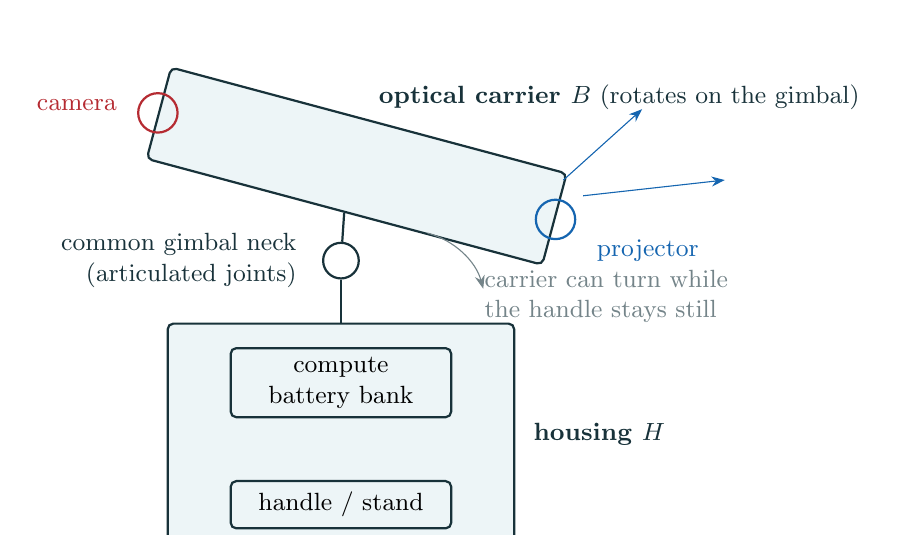
\begin{tikzpicture}[font=\small,
  box/.style={draw=ink,thick,rounded corners=2pt,fill=paperblue,
    align=center},
  joint/.style={circle,draw=ink,thick,fill=white,inner sep=1.6mm}]
  % housing
  \node[box,minimum width=44mm,minimum height=28mm] (house) at (0,-0.6) {};
  \node[box,minimum width=28mm] at (0,0.05) {compute\\ battery bank};
  \node[box,minimum width=28mm,minimum height=6mm] at (0,-1.5)
    {handle / stand};
  \node[ink,anchor=west] at (house.east) {\ \textbf{housing $H$}};
  % gimbal neck
  \node[joint] (g) at (0,1.6) {};
  \draw[ink,thick] (house.north) -- (g);
  \node[ink,anchor=east,align=right] at ([xshift=-2mm]g.west)
    {common gimbal neck\\ (articulated joints)\ };
  % optical carrier
  \node[box,minimum width=52mm,minimum height=12mm,rotate=-15]
    (carrier) at (0.2,2.8) {};
  \draw[ink,thick] (g) -- (carrier.south);
  \node[circle,draw=HW,thick,minimum size=5mm] at (carrier.west) {};
  \node[circle,draw=IO,thick,minimum size=5mm] at (carrier.east) {};
  \node[HW,anchor=east] at ([xshift=-4mm,yshift=1mm]carrier.west) {camera};
  \node[IO,anchor=west] at ([xshift=4mm,yshift=-4mm]carrier.east)
    {projector};
  \draw[-{Stealth},IO] (carrier.east) ++(0.1,0.5) -- ++(1.0,0.9);
  \draw[-{Stealth},IO] (carrier.east) ++(0.35,0.3) -- ++(1.8,0.2);
  \node[ink,anchor=south west] at (carrier.north)
    {\textbf{optical carrier $B$} (rotates on the gimbal)};
  \draw[-{Stealth},ink!60] (1.1,1.95) arc[start angle=75,end angle=15,
    radius=10mm];
  \node[ink!60,anchor=west,align=left] at (1.7,1.15)
    {carrier can turn while\\ the handle stays still};
\end{tikzpicture}
\end{center}
Schematic component layout, not an optical ray diagram: both the camera
and the projector face the working area. The camera and projector move
\textbf{together} on the carrier; neither keeps a fixed offset to the
housing while the gimbal turns. A parked
lantern whose joints are locked behaves like a static projector; a parked
housing with moving joints does not.
Figure~\ref{fig:lantern-loops} sketches the three cooperating loops that
keep such a lantern honest.

\begin{plain}{A good first demonstration}
Start with one room-locked surface, one fixed projector, one moving
camera--projector pair on a carried lantern's gimballed carrier, and a
fixed FF. Prove agreement on that surface before adding a second moving
lantern, smoke, or neural prediction.
\end{plain}

\begin{center}
\begin{minipage}{\linewidth}
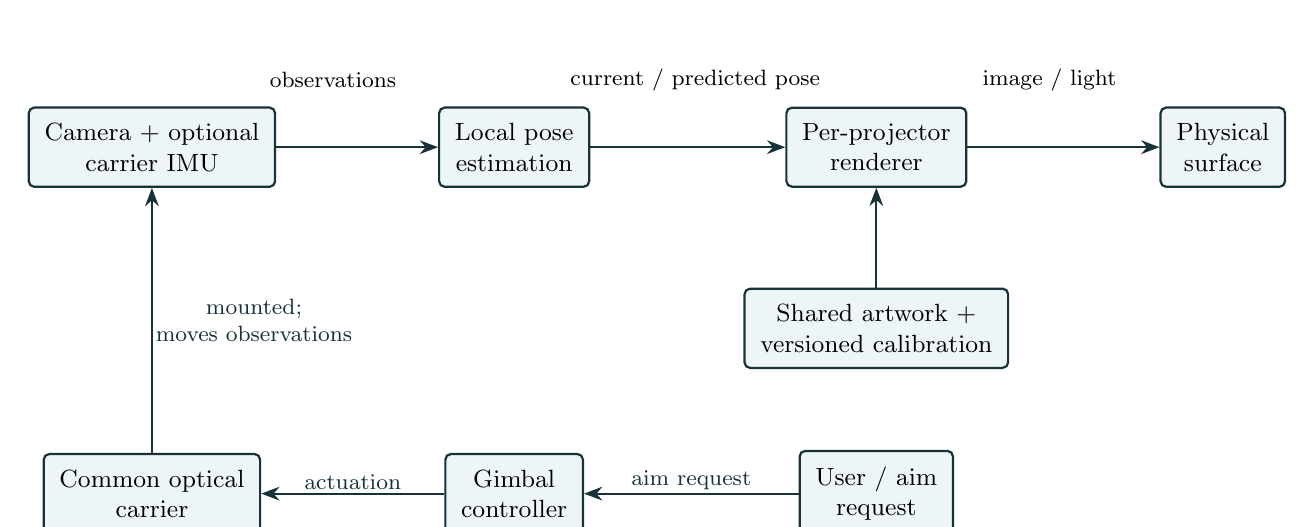
\begin{tikzpicture}
  \node[flow] (cam) at (0,0) {Camera + optional\\ carrier IMU};
  \node[flow] (pose) at (4.6,0) {Local pose\\ estimation};
  \node[flow] (ren) at (9.2,0) {Per-projector\\ renderer};
  \node[flow] (surf) at (13.6,0) {Physical\\ surface};
  \draw[edge] (cam) -- (pose);
  \draw[edge] (pose) -- (ren);
  \draw[edge] (ren) -- (surf);
  \node[flab] at (2.3,0.85) {observations};
  \node[flab] at (6.9,0.85) {current / predicted pose};
  \node[flab] at (11.4,0.85) {image / light};
  \node[flow] (pipe) at (9.2,-2.3) {Shared artwork +\\ versioned calibration};
  \draw[edge] (pipe.north) -- (ren.south);
  \node[flow] (carr) at (0,-4.4) {Common optical\\ carrier};
  \node[flow] (ctl) at (4.6,-4.4) {Gimbal\\ controller};
  \node[flow] (user) at (9.2,-4.4) {User / aim\\ request};
  \draw[edge] (user) -- node[flab,above]{aim request} (ctl);
  \draw[edge] (ctl) -- node[flab,above]{actuation} (carr);
  \draw[edge] (carr) -- node[flab,right]{mounted;\\ moves observations}
    (cam.south);
\end{tikzpicture}
\captionof{figure}{The gimbal moves the optical platform; sensing
estimates its actual pose; rendering places the artwork. The shared pipe
supplies artwork and calibration, not magical localization. This is
conceptual control/data flow, not electrical wiring.}
\label{fig:lantern-loops}
\end{minipage}
\end{center}

\section{Audit: Keep the Vision, Remove the Impossible Promises}
\label{sec:audit}

Source keys S1--S9 refer to the exact supplied filenames in
Section~\ref{sec:sources}. These documents are design inputs, not independent
experimental evidence. Their placeholder references such as
\texttt{[cite: 2]} are not traceable publications and are not retained as proof.

\small
\begin{longtable}{@{}L{25mm}L{56mm}L{74mm}@{}}
\toprule
Verdict & Claim in the inputs & Correction / consequence\\
\midrule
\endfirsthead
\toprule Verdict & Claim in the inputs & Correction / consequence\\ \midrule
\endhead
\bottomrule\endfoot
Critical / S6 &
Detect a marker ID and fetch the master transform; no local geometry solve. &
ID gives identity, not six-dimensional pose. A device still needs calibrated
image corners and a pose solve, an existing local map aligned to the world,
or an external pose measurement. A server may solve remotely, but the
measurement and time alignment do not disappear.\\
Critical / S5 &
An FF observation distinguishes an FF move from a bumped camera. &
It measures their relative pose only. A trusted fixed landmark, fixed
camera, or independently world-aligned tracker is required to attribute
motion. All devices and the FF can otherwise drift together.\\
Critical / S2--S4 &
Interpolation and NPU prediction eliminate latency and guarantee 60 Hz. &
Interpolation needs bracketing samples and therefore usually a delay.
Extrapolation estimates the future and can be wrong. A worker protects the
render thread but cannot guarantee GPU deadlines or light-emission timing.\\
Critical / S1, S8 &
High-intensity/IR countermeasures aimed at eyewear; a shutter guarantees safety. &
Exclude targeted sensor-blinding from the artistic system. Do not aim at
eyes or faces. Black pixels, software masks, and generic privacy/welding
films are not certified optical safety shutters. A handheld beam can still
sweep a bystander; assess the complete optical system before use around
people.\\
Major / S9 &
FF height is 100 mm; rank-three face normals guarantee a positive-definite
pose Hessian and no depth ambiguity. &
The repository's measured v1 height is 42.5 mm. Normals alone do not prove
pose observability. Visible corner layout, image size, viewing angle,
intrinsics and noise determine conditioning. A planar target can yield a
valid calibrated pose; non-planarity is helpful, not magical.\\
Major / S2--S5 &
Stage FF is 5 m wide, so scale and occlusion are solved. &
This is a proposed different artifact, with no supplied height or measured
marker layout. It needs its own surveyed model. Larger targets can help
pixel coverage but do not remove occlusion or motion blur.\\
Major / S2--S5, S8 &
Translation in $[R\mid t]$ is the camera's world position; pointing
direction determines orientation. &
For world-to-camera extrinsics the center is $-R^\top t$.
A direction omits roll: give a full rotation or a nonparallel up direction.\\
Major / S7 &
\texttt{solvePnP} estimates lens distortion as well as pose. &
Standard PnP takes $K$ and distortion as inputs and estimates rotation and
translation. Intrinsic/distortion calibration is a separate, sufficiently
excited multi-view optimization.\\
Major / S2--S6 &
One nearby marker is equivalent to the full non-planar target. &
A known square can support pose, but is planar, often ambiguous/noisy,
especially small or front-facing. Use candidate poses, positive depth,
temporal/IMU evidence and uncertainty; fall back to more landmarks.\\
Major / S8, S9 &
One homography aligns all 3D artwork from any moving viewpoint. &
A homography is exact only for a plane in undistorted pinhole coordinates
(or special pure-rotation view changes). Multiple depths need per-surface
maps or full 3D rendering and depth tests.\\
Major / S5, S6 &
An IMU/Myo supplies a world-space ray origin; a phone's known position
alone can recalibrate a camera. &
An IMU measures rotation rate and specific force, not absolute position.
A ray needs a known origin. A phone must expose enough measured visual
geometry with known pose; an invisible network pose is not a correspondence.\\
Major / S1, S8 &
Beams meeting in smoke form a stable free-floating 3D canvas. &
Haze scatters along entire beams; rays continue beyond their crossing.
Conventional projectors do not selectively illuminate arbitrary isolated
voxels. Treat smoke as a beam sculpture, not a volumetric display.\\
Major / S1, S8 &
Two projectors automatically double usable brightness; overlap is fixed
at a sweet-spot distance. &
Irradiances add only where footprints meet. Calibrated rendering can align
on known surfaces at many distances, but overlap, focus, falloff, black
level, occlusion and eye safety still constrain the result.\\
Major / S1, S8 &
A 65/100 W bank and generic 12 V trigger guarantee two-projector operation. &
Total wattage does not specify per-port voltage/current, simultaneous
profiles, startup peaks or thermal derating. Check exact modules, cable
rating and negotiated profiles; do not assume 12 V PD exists.\\
Unproven / S1, S8, S9 &
Millimetre/sub-millimetre alignment and a fixed affordable bill of materials. &
These are targets, not measurements. Specify range, pixel coverage,
static/dynamic error and percentiles; include optics, cooling, mounts,
safety, cables, power conversion and local price verification.\\
Keep / S2--S8 &
Local rendering, a shared spatial pipe, asynchronous tracking and simple
vector art. &
Strong architecture once every transform has a direction, timestamp,
revision and uncertainty, and the system defines failure behavior.
Simple visuals reduce visual sensitivity but do not correct bad geometry.\\
\end{longtable}
\normalsize

\section{The Language: Rulers, Places, and Directions}
\label{sec:notation}

\begin{plain}{A coordinate frame is a labelled ruler}
A frame says where zero is and which directions count as right, forward,
and up. The same physical point has different numbers when measured from
the room, the FF, or a camera. A transform translates between those rulers;
it does not move the physical point.
\end{plain}

\subsection{Conventions fixed before any equation}
Use column vectors, right-handed frames, metres, seconds and radians.
The existing repository uses millimetres for FF geometry/extrinsics:
\textbf{convert at the interface}, not halfway through a matrix product.
Pixel coordinates are in pixels, with $u$ to the right and $v$ down.

The room frame is $W$, chosen once per session; its $+z$ is up.
The FF frame is $F$, centered on its base, with $+z$ up.
$C_i$ names camera $i$, $D_i$ a depth camera, $P_j$ projector $j$,
$B$ a rigid moving body---in the lantern design this is the gimballed
\emph{optical carrier}---$H$ the lantern \emph{housing} frame when a
lantern is present, and $M_k$ a known marker.
An optical device's axes follow OpenCV: $+x$ right, $+y$ down, $+z$ forward.
The carrier's axes may differ from the housing's; document both.
Where the letter $H$ appears as a filter observation Jacobian, context
keeps it distinct from the housing frame.

\begin{longtable}{@{}L{34mm}L{125mm}@{}}
\toprule Symbol & Meaning and shape\\ \midrule
\endfirsthead
\toprule Symbol & Meaning and shape\\ \midrule \endhead
\bottomrule\endfoot
$t$, $\Delta t$ & Time and elapsed time, in seconds. A bold $\bm{t}$ below
is a translation vector, not time.\\
$\pt{A}$, $\hpt{A}$ & A point measured in frame $A$, a $3\times1$ vector,
and the same point with a final 1 appended, a $4\times1$ vector.\\
$\T{A}{B}(t)$ & A $4\times4$ transform taking coordinates \emph{from $B$ to $A$}.
Read the arrow literally. $A,B$ here are any named frames.\\
$\Rot{A}{B}$, $\tr{A}{B}$ & Its $3\times3$ rotation and $3\times1$ translation.\\
$I$, $\bm{0}$, $(\cdot)^\top$ & Identity matrix, zero vector/matrix,
and transpose; dimensions follow the surrounding equation.\\
$\bm{c}_W$, $\bm{p}_W$ & An optical device's center and unit forward
direction, both expressed in the room. These are not extrinsic translation.\\
$w_V,h_V,K_V,\bm{d}_V$ & Device $V$'s width, height, intrinsic matrix,
and distortion coefficients. $V$ can be any camera or projector.\\
$\bm{q}=(u,v)^\top$, $\bar{\bm{q}}=(u,v,1)^\top$ &
A measured image pixel and its homogeneous form.\\
$\pi_V(\pt{V})$ & The complete projection recipe for device $V$:
divide by depth, distort, then apply intrinsics.\\
$\|\bm{a}\|$, $\bm{a}\times\bm{b}$ &
Euclidean length and three-dimensional cross product.\\
$\hat{\phantom{x}}$, $^-$, $^+$ & Estimated quantity, estimate before
a measurement correction, estimate after correction.\\
$\Sigma$, $P$, $Q$, $N$ & Measurement covariance, state-error covariance,
process-noise covariance, and measurement-noise covariance in the filter.
Projector symbols have an indexed $P_j$, not an unindexed covariance $P$.\\
\end{longtable}
Additional symbols are introduced next to their first equation. A covariance
describes uncertainty and correlations, not a generic ``confidence score.''

\subsection{The one transform rule to remember}
A rotation turns a direction; a translation shifts a point:
\begin{equation}
\pt{A}=\Rot{A}{B}\pt{B}+\tr{A}{B},\qquad
\hpt{A}=\T{A}{B}\hpt{B},\qquad
\T{A}{B}=
\begin{bmatrix}\Rot{A}{B}&\tr{A}{B}\\\bm{0}^\top&1\end{bmatrix}.
\label{eq:transform}
\end{equation}
A proper rotation has $R^\top R=I$ and $\det R=+1$.
These rotations form the set $SO(3)$; the rigid transforms form $SE(3)$.
Those names mean ``legal rotations'' and ``legal rotation-plus-translation
recipes,'' not additional hardware.

To chain transforms, match the inner frame names. To reverse a transform,
undo the translation in the rotated coordinates:
\begin{equation}
\T{A}{C}=\T{A}{B}\T{B}{C},\qquad
\T{B}{A}=\T{A}{B}^{-1}
=\begin{bmatrix}R^\top&-R^\top\bm{t}\\\bm{0}^\top&1\end{bmatrix}.
\label{eq:compose}
\end{equation}
Here $R=\Rot{A}{B}$ and $\bm{t}=\tr{A}{B}$. Products are evaluated
right to left. At live time, all dynamic factors must refer to the
\textbf{same physical time}, not simply their latest arrival times.

\subsection{Where a camera really is}
For world-to-camera extrinsics $R=\Rot{C}{W}$, $\bm{t}=\tr{C}{W}$,
the camera center and its pointing direction in the world are
\begin{equation}
\bm{c}_W=-R^\top\bm{t},\qquad
\bm{p}_W=R^\top(0,0,1)^\top.
\label{eq:center}
\end{equation}
Why? The camera's own center has coordinates $\bm{0}$ in camera space.
Substitute that into Equation~\eqref{eq:transform} and solve backwards.
Its translation $\bm{t}$ instead tells us where the \emph{world origin}
appears in the camera.

For a human-friendly ``look at'' pose, specify center $\bm{c}_W$,
unit forward $\bm{f}$ and an approximate world-up vector $\bm{u}$ that is
not parallel to $\bm{f}$. Define right $\bm{r}$ and down $\bm{b}$:
\begin{equation}
\bm{r}=\frac{\bm{f}\times\bm{u}}{\|\bm{f}\times\bm{u}\|},
\quad \bm{b}=\bm{f}\times\bm{r},\quad
R=\begin{bmatrix}\bm{r}^\top\\\bm{b}^\top\\\bm{f}^\top\end{bmatrix},
\quad \bm{t}=-R\bm{c}_W.
\end{equation}
If looking straight up/down, choose a different nonparallel reference-up.
That choice fixes roll; pointing alone never does.

\section{The Lens Recipe: From a Point to a Pixel}
\label{sec:lens}

\subsection{Perspective, intrinsics and distortion}
Let $\pt{V}=(X,Y,Z)^\top$ be a point in device $V$.
Only $Z>0$ is in front of the lens. Normalize by depth:
$x=X/Z$, $y=Y/Z$. These $x,y$ are dimensionless.
Let $f_x,f_y$ be focal lengths in pixels, $c_x,c_y$ the principal point,
and $\gamma$ pixel-axis skew (normally fixed to zero):
\begin{equation}
K_V=\begin{bmatrix}f_x&\gamma&c_x\\0&f_y&c_y\\0&0&1\end{bmatrix}.
\end{equation}
For the common five-coefficient OpenCV lens model, store
$\bm{d}_V=(k_1,k_2,p_1,p_2,k_3)$ \emph{in that order}. With squared
radius $r^2=x^2+y^2$ and radial factor $a$, the full recipe is
\begin{align}
a&=1+k_1r^2+k_2r^4+k_3r^6,\\
x_d&=xa+2p_1xy+p_2(r^2+2x^2),\\
y_d&=ya+p_1(r^2+2y^2)+2p_2xy,\\
\pi_V(X,Y,Z)&=
\begin{bmatrix}f_xx_d+\gamma y_d+c_x\\f_yy_d+c_y\end{bmatrix}.
\label{eq:projection}
\end{align}
Fisheye lenses need a matching fisheye model; do not reinterpret their
coefficients as these five numbers.

\begin{plain}{Perspective is a divide, not a mysterious squash}
A point twice as far away has half the image displacement from the
principal point. The matrix sets the ruler in pixels; distortion bends that
ideal ruler. Use the same recipe for solving and for drawing the overlay.
\end{plain}

With no distortion, the compact homogeneous equation is
\begin{equation}
Z\bar{\bm{q}}=K_V
\begin{bmatrix}\Rot{V}{W}&\tr{V}{W}\end{bmatrix}\hpt{W}.
\end{equation}
The multiplier is device-space depth for this normalization. The final
division by the third coordinate is essential. With distortion, use
Equation~\eqref{eq:projection}, not this matrix alone.

\subsection{Resolution changes, cropping and automatic optics}
For a pure coordinate resize $u'=s_xu$, $v'=s_yv$,
\begin{equation}
K'=\operatorname{diag}(s_x,s_y,1)K,\qquad \bm{d}'=\bm{d}.
\label{eq:resize}
\end{equation}
For cropping by offsets $u_0,v_0$ before resizing, use
$c_x'=s_x(c_x-u_0)$, $c_y'=s_y(c_y-v_0)$.
Some resamplers map pixel centers as
$u'=s_x(u+1/2)-1/2$; then the same offset belongs in $c_x'$.
Record the actual sampling convention and full image preprocessing map.
Rotation, mirroring, stabilization, digital zoom and keystone are not
automatically described by simple focal-length scaling.

Lock optical zoom/focus where possible. Disable auto-keystone, obstacle
avoidance, auto-fit, and changing digital stabilization for a calibrated
projector. A calibrated, fixed warp can be explicitly modeled, but an
unknown changing warp invalidates the model. Recheck intrinsics after an
optical focus/zoom change; a digital focus command is not a pose update.

\subsection{Example 1: A deliberately tiny $32\times16$ image}
This is an arithmetic aid, \textbf{not} enough resolution for practical FF
tracking. Choose zero distortion and
\begin{equation}
K=\begin{bmatrix}16&0&16\\0&16&8\\0&0&1\end{bmatrix},\qquad
K^{-1}=\begin{bmatrix}1/16&0&-1\\0&1/16&-1/2\\0&0&1\end{bmatrix}.
\label{eq:tinyK}
\end{equation}
Our continuous image coordinates have bounds $[0,32)\times[0,16)$.
The principal point is chosen as $(16,8)$; real principal points are
measured, not forced to the midpoint. Horizontal field of view is
$2\arctan(32/(2\cdot16))=90^\circ$; vertical is about $53.13^\circ$,
\emph{not} $90^\circ$.

For $\pt{C}=(0.25,0.125,1)$ metres, normalized coordinates are
$(0.25,0.125)$, so $\bm{q}=(20,10)$ pixels.
Conversely $(20,10)$ identifies the ray
$K^{-1}(20,10,1)^\top=(0.25,0.125,1)^\top$, not a unique point:
depth or a surface is still missing.

\section{What the FF Measures, and What PnP Actually Solves}
\label{sec:pnp}

\subsection{Use the built artifact, not a convenient ideal pyramid}
For the repository's \textbf{v1 physical FF}, base edge $b=0.155$ m,
top edge $a=0.075$ m, height $h=0.0425$ m.
Top marker ID 10 is 0.055 m square; side markers 11--14 are 0.050 m.
The dictionary is \texttt{DICT\_4X4\_50}; IDs 11,12,13,14 label
$+y,+x,-y,-x$, respectively.

Base vertices are $(\pm b/2,\pm b/2,0)$; top vertices are
$(\pm a/2,\pm a/2,h)$. Let inset $s=(b-a)/2=0.040$ m.
The slope angle \emph{above horizontal} is $\arctan(h/s)\simeq46.736^\circ$.
For example the outward $+y$ side normal is
\begin{equation}
\bm{n}_{+y}=\frac{(0,h,s)^\top}{\sqrt{h^2+s^2}}
\simeq(0,0.72820,0.68536)^\top.
\end{equation}
The top marker's corners, in decoded top-left, top-right, bottom-right,
bottom-left order, are
\begin{equation}
\begin{bmatrix}
-0.0275& 0.0275&0.0425\\
 0.0275& 0.0275&0.0425\\
 0.0275&-0.0275&0.0425\\
-0.0275&-0.0275&0.0425
\end{bmatrix}\ {\rm m}.
\end{equation}
Rows list points; the transform equations still use column vectors.
Use all side-marker corners from \texttt{fulcrum\_spec.json}, divided by
1000, rather than inferring sticker positions from face dimensions.
The file notes an assumed, unmeasured 4 mm sticker gap and has an older
``about 45 mm'' height note: re-survey the real object before asserting
sub-millimetre accuracy. The measured block's current height is 42.5 mm.

The proposed 5 m stage object in S2--S5 has no complete supplied survey.
It is not a scaled copy of this artifact unless explicitly built and measured
as such. Also distinguish these \emph{document revisions} from the repository's
\texttt{ffv2\_spec.json}, which describes a separate painted tracking solid.

\subsection{The correspondence contract}
For each visible marker corner $i$, take the known point $\pt{F,i}$ from
the model and its detected image point $\bm{q}_{C,i}$.
Match marker identity \emph{and decoded corner order}.
Knowing the printed size alone is insufficient if its placement on the
FF is unknown. Never sort corners only by screen $x$ or $y$.

Let $\mathcal{I}$ be the accepted corner indices.
PnP estimates a pose $\T{C}{F}$ with fixed $K_C,\bm{d}_C$:
\begin{equation}
(\hat R,\hat{\bm{t}})
=\argmin_{R\in SO(3),\,\bm{t}}
\sum_{i\in\mathcal I}
\rho\!\left(
\bm{e}_i^\top\Sigma_i^{-1}\bm{e}_i
\right),\qquad
\bm{e}_i=\bm{q}_{C,i}-\pi_C(R\pt{F,i}+\bm{t}).
\label{eq:pnp}
\end{equation}
Here $\bm{e}_i$ is a two-pixel-component residual; $\Sigma_i$ is its
$2\times2$ covariance; $\rho$ is a robust loss that reduces outlier influence.
This is a \emph{desired robust objective}, not a statement that ordinary
\texttt{solvePnP} automatically implements Huber loss or covariance weighting.
Use a robust wrapper/RANSAC to reject bad correspondences, then refine
and re-evaluate all accepted observations.

\textbf{Outputs.} OpenCV returns a rotation vector \texttt{rvec} and
translation \texttt{tvec}, taking FF points \emph{into camera space}.
Convert rotation using \texttt{cv2.Rodrigues}. If $\bm{\theta}$ is a
rotation vector, $\theta=\|\bm{\theta}\|$ its angle and
$\bm{a}=\bm{\theta}/\theta$ its axis, then
\begin{equation}
R=I+\sin\theta\,\sk{\bm{a}}+(1-\cos\theta)\sk{\bm{a}}^2,\qquad
\sk{\bm{a}}=
\begin{bmatrix}0&-a_z&a_y\\a_z&0&-a_x\\-a_y&a_x&0\end{bmatrix}.
\end{equation}
Use the zero-angle limit $R=I$. A quaternion is another orientation
representation; state its component order and normalize it. Do not average
rotation matrices or quaternion components as if they were positions.

\subsection{Ambiguity, conditioning, and honest quality}
A single square supplies four coplanar corners and can support pose with
known intrinsics; it may yield competing or weakly separated solutions.
IPPE-style planar candidate evaluation is useful.
Non-coplanar visible corners help, but a solver's minimal point count is
not a production-quality acceptance rule.

Require positive depths, enough image spread, plausible motion, and agreement
with independent observations. The offline repository registration requests
at least three FF markers; its TD live path can use two, or one during
short-term tracking with a prior. Those paths do not have equal certainty.
Do not promote a one-marker continuation to a fresh global registration.

For local pose perturbations $\delta\bm{\xi}$ (three translation and three
rotation components), let $J$ be the Jacobian of residuals with respect to
those six components and let $W_e$ be their inverse-covariance weighting.
Under a locally Gaussian, well-conditioned approximation,
\begin{equation}
\Sigma_{\xi}\simeq(J^\top W_eJ)^{-1}.
\label{eq:posecov}
\end{equation}
Near-singularity means uncertainty is large; do not silently invert it and
claim precision. This local formula omits lens and model error unless those
uncertainties are included. Face-normal rank is \emph{not} a proof about
$J^\top W_eJ$.

Report per-view RMS pixel error
$e_{\rm RMS}=\sqrt{\sum_i\|\bm{e}_i\|^2/|\mathcal I|}$,
maximum error, marker coverage, age, and independent surface alignment.
Mean corner distance and RMS are different metrics. Low in-sample
reprojection error alone does not prove correct world anchoring.
At focal length 1000 px and distance 5 m, a 50 mm marker is only about
10 px wide before foreshortening: that is a warning, not a reliable
room-scale reference.

\subsection{Lens calibration is a different optimization}
Before live pose tracking, collect diverse views over the lens field,
with different tilts, distances, and adequate lighting. Let $k$ index
views, $i$ corners, and $R_k,\bm{t}_k$ each target-to-camera pose.
Estimate shared lens parameters along with separate per-view poses:
\begin{equation}
\argmin_{K,\bm{d},\{R_k,\bm{t}_k\}}
\sum_{k,i}\rho\!\left(
\|\bm{q}_{ki}-\pi_{K,\bm{d}}(R_k\pt{F,i}+\bm{t}_k)\|^2
\right).
\label{eq:lensfit}
\end{equation}
\texttt{calibrateCamera} and suitable calibration tools support this class
of problem. Priors and held-out views help prevent overfitting.
One small FF at one image location cannot reliably constrain all distortion
parameters. Lock intrinsics for routine live PnP; motion usually requires a
new pose, not a new lens fit.

\section{The Shared World: Initial Registration and Moving Anchors}
\label{sec:world}

\begin{plain}{The FF can be a ruler without being the room}
At setup, you may declare ``the FF's current base is the room origin.''
Afterwards the room ruler stays put. The physical FF may move.
Artwork attached to the FF follows it; artwork attached to the room does not.
Someone must keep observing the relation between those two rulers.
\end{plain}

\subsection{Initial fixed-FF registration}
At setup time $t_0$, hold the FF still and choose $\T{W}{F}(t_0)$.
The simplest choice is $I$: the room agrees with the FF \emph{at that instant}.
For every camera seeing it,
\begin{equation}
\T{W}{C_i}(t_0)=
\T{W}{F}(t_0)\T{C_i}{F}(t_0)^{-1}.
\label{eq:initial}
\end{equation}
For a genuinely fixed camera, retain this world pose while its mount remains
unchanged. Simultaneous observations of a fixed FF give the camera-to-camera
registration
\begin{equation}
\T{C_i}{C_j}=
\T{C_i}{F}\T{C_j}{F}^{-1}.
\label{eq:paired}
\end{equation}
Sequential captures are acceptable only while the FF \emph{and both cameras}
are still. The term ``paired'' does not itself mean hardware synchronized.

\subsection{A moving FF with an independent fixed reference}
Let $C_s$ be a trusted static camera with known $\T{W}{C_s}$.
It observes the moving FF:
\begin{equation}
\T{W}{F}(t)=\T{W}{C_s}\T{C_s}{F}(t).
\label{eq:movingff}
\end{equation}
A moving camera $C_m$ also sees the FF at that same time:
\begin{equation}
\T{W}{C_m}(t)=
\T{W}{F}(t)\T{C_m}{F}(t)^{-1}.
\label{eq:movingcam}
\end{equation}
This is the general live-recalibration equation. It requires
\emph{independent knowledge} of $\T{W}{F}(t)$.
If only FF-relative artwork matters, a camera--projector pair can operate
directly in $F$ without a persistent room frame.

\subsection{Why a lone moving FF is not enough}
The observation relation is
$\T{C}{F}=\T{W}{C}^{-1}\T{W}{F}$.
For any common world transform $G(t)$,
\begin{equation}
\bigl(G(t)\T{W}{C}(t)\bigr)^{-1}
\bigl(G(t)\T{W}{F}(t)\bigr)
=\T{W}{C}(t)^{-1}\T{W}{F}(t).
\label{eq:gauge}
\end{equation}
The image cannot distinguish these alternatives.
This unobservable freedom is often called \emph{gauge freedom}.
It is why a low residual cannot tell whether the FF moved, the camera moved,
or both moved together.

Provide a surveyed static marker network, a trusted fixed camera, or a
VIO/SLAM map aligned to $W$ to preserve room-lock. If all absolute references
are lost, publish \texttt{relative-only} or growing uncertainty, not a
fictional fully tracked room pose. Multiple cameras help only when they
connect to independent constraints; a circle of mutually derived estimates
does not create new evidence.

\subsection{Distributed local maps and marker relays}
Suppose a phone tracks in local map $L$, and that map provides
$\T{L}{C}(t)$. A known world marker $M$ is observed with PnP
$\T{C}{M}(t)$, and its world pose $\T{W}{M}(t)$ is known.
Align the map once, then update as needed:
\begin{equation}
\T{W}{L}=
\T{W}{M}(t)
\bigl(\T{L}{C}(t)\T{C}{M}(t)\bigr)^{-1},\qquad
\T{W}{C}=\T{W}{L}\T{L}{C}.
\label{eq:mapalign}
\end{equation}
This is the valid version of ``detect and align.'' It still needs the
camera's observation or an existing pose, that camera's own intrinsics,
and a known marker pose at the capture time. There is no universal
\texttt{K\_master} suitable for every device.

A tracked phone can serve as a relay only if another camera observes
known-size, known-pose geometry attached to it (for example a calibrated
marker), at an aligned time. Network position alone is not visible evidence.

\subsection{Example 2: A moved FF does not move the room}
Use metres and a camera looking straight down from $(0,0,1)$:
\begin{equation}
R=\operatorname{diag}(1,-1,-1),\quad
\T{C}{W}=
\begin{bmatrix}1&0&0&0\\0&-1&0&0\\0&0&-1&1\\0&0&0&1\end{bmatrix}.
\end{equation}
Move the FF without rotation to world position $(0.2,0.1,0)$.
Then
\begin{equation}
\T{W}{F}=
\begin{bmatrix}1&0&0&0.2\\0&1&0&0.1\\0&0&1&0\\0&0&0&1\end{bmatrix},
\qquad
\T{C}{F}=
\begin{bmatrix}1&0&0&0.2\\0&-1&0&-0.1\\0&0&-1&1\\0&0&0&1\end{bmatrix}.
\end{equation}
The camera's FF-relative center becomes $(-0.2,-0.1,1)$.
Equation~\eqref{eq:movingcam} still gives its world center $(0,0,1)$.
A point at the FF origin moves to $(0.2,0.1,0)$; a previously room-locked
point at $(0,0,0)$ stays there.

For the same overhead camera and the FF at the initial origin, the four
top-marker pixels using Equation~\eqref{eq:tinyK} are approximately
$(15.54047,7.54047)$, $(16.45953,7.54047)$,
$(16.45953,8.45953)$, $(15.54047,8.45953)$.
All have positive camera depth $1-0.0425=0.9575$ m.
This tiny square illustrates why the $32\times16$ example is not a practical
tracking configuration.

\section{Projectors: Fixed Lights and Gimballed Projection Lanterns}
\label{sec:projectors}

\subsection{The projector is an inverse camera, not a camera sensor}
For a world surface point, decide which projector pixel should illuminate it:
\begin{equation}
\bm{q}_{P_j}(t)=
\pi_{P_j}\!\left(\T{P_j}{W}(t)\hpt{W}(t)\right).
\label{eq:projector}
\end{equation}
In this and subsequent shorthand, $\pi$ takes the first three components
of the transformed homogeneous point.
Use only points in front of the lens and inside the output image.
Clip triangles crossing the near plane; test the nearest surface along
each projector ray with a depth buffer or mesh intersection.

A projector cannot see printed markers. To calibrate it:
\begin{enumerate}
  \item Calibrate a camera and determine its pose relative to a known surface,
    FF, or independently measured 3D model.
  \item Project identifiable patterns at known \emph{projector pixels}.
    Use Gray codes, indexed dots, or distinguishable projected markers.
  \item Observe the lit pixels in the camera; invert camera distortion and
    intersect their rays with known surfaces, use registered depth, or
    triangulate with synchronized calibrated cameras.
  \item Pair those recovered 3D points with their known projector pixels.
    With known projector intrinsics, solve projector PnP. For unknown lens
    parameters, gather diverse geometry/views and calibrate them separately.
  \item Validate on different points, depths, and image regions. A single
    plane gives a homography, not a fully constrained arbitrary projector
    lens/distortion calibration.
\end{enumerate}
Do not derive unknown surfaces from the same unverified projector model
and then call them independent validation. Isolate multiple projectors'
patterns by time or coding; otherwise a camera may match the wrong emitter.

\subsection{The lantern has two moving parts, not one rigid pose}
\begin{plain}{One handle, one articulated neck, one optical platform}
The lantern's outer housing holds the handle, compute, power bank and
gimbal base. A common gimbal carries the camera and projector together
on a rigid optical platform. You can move the handle while that platform
holds its aim, or turn the platform while the handle stays still.
The camera and projector keep their mutual offset; neither keeps a fixed
offset to the handle while the gimbal turns.
\end{plain}

Let $H$ name the lantern \emph{housing} frame, and $B$ the gimballed
\emph{optical carrier} frame. Throughout the lantern model, $B$ refers to
this optical carrier, not the housing.
Let $\bm{\alpha}=(\alpha_1,\ldots,\alpha_r)$ be the actual measured angles
of $r$ gimbal joints, in radians, after encoder zero-offset correction.
A two- or three-axis gimbal is allowed; its joint order, axes, pivots,
signs and angle limits are calibration data.

The fixed mounting transforms are $\T{B}{C}$ and $\T{B}{P}$.
The articulated transform $\T{H}{B}(\bm{\alpha})$ changes with the joints.
The world camera and projector poses follow the complete chain:
\begin{align}
\T{W}{B}(t)&=\T{W}{H}(t)\T{H}{B}(\bm{\alpha}(t)),\\
\T{W}{C}(t)&=\T{W}{B}(t)\T{B}{C},\\
\T{W}{P}(t)&=\T{W}{B}(t)\T{B}{P},\qquad
\T{P}{C}=\T{B}{P}^{-1}\T{B}{C}.
\label{eq:rig}
\end{align}
Thus the camera-to-projector transform is constant even though the
camera-to-housing and projector-to-housing transforms are not.
For a parked lantern, its housing may be static while its projector is
still moving. Only a fixed housing \emph{and locked joints} make the
whole lantern equivalent to a static projector.
Figure~\ref{fig:lantern-frames} draws these links as a coordinate
transform graph.

\begin{center}
\begin{minipage}{\linewidth}
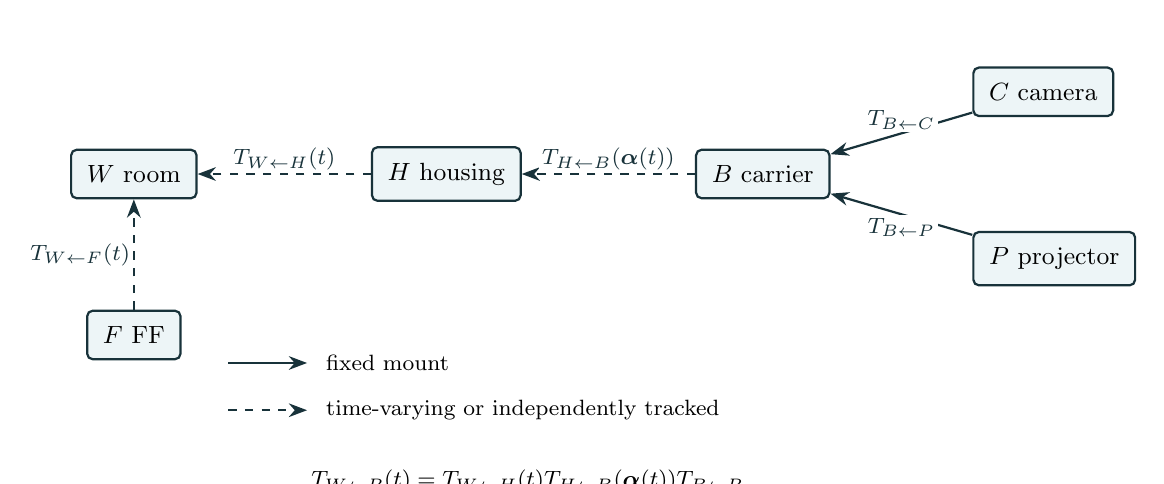
\begin{tikzpicture}[node distance=5mm and 16mm]
  \node[flow] (W) {$W$ room};
  \node[flow,right=22mm of W] (H) {$H$ housing};
  \node[flow,right=22mm of H] (B) {$B$ carrier};
  \node[flow,above right=4mm and 18mm of B] (C) {$C$ camera};
  \node[flow,below right=4mm and 18mm of B] (P) {$P$ projector};
  \node[flow,below=14mm of W] (F) {$F$ FF};
  \draw[dedge] (H) -- node[flab,above]{$\T{W}{H}(t)$} (W);
  \draw[dedge] (B) -- node[flab,above]{$\T{H}{B}(\bm{\alpha}(t))$} (H);
  \draw[edge] (C) -- node[flab,above]{$\T{B}{C}$} (B);
  \draw[edge] (P) -- node[flab,below]{$\T{B}{P}$} (B);
  \draw[dedge] (F) -- node[flab,left]{$\T{W}{F}(t)$} (W);
  \draw[edge] (1.2,-2.4) -- (2.2,-2.4);
  \node[flab,anchor=west] at (2.4,-2.4) {fixed mount};
  \draw[dedge] (1.2,-3.0) -- (2.2,-3.0);
  \node[flab,anchor=west] at (2.4,-3.0) {time-varying or
    independently tracked};
  \node[flab] at (5.0,-3.9)
    {$\T{W}{P}(t)=\T{W}{H}(t)\T{H}{B}(\bm{\alpha}(t))\T{B}{P}$};
\end{tikzpicture}
\captionof{figure}{Arrows map point coordinates from the tail frame into
the head frame; they are not motion or network arrows. Read a
projector-to-world chain from right to left. The camera and projector
share fixed carrier mounts, while the housing--carrier link changes as
the joints turn.}
\label{fig:lantern-frames}
\end{minipage}
\end{center}

\subsection{Two valid ways to know where the light is}
\textbf{Route A: track the optical carrier directly.}
The camera rides on the carrier and sees the FF.
With an independently known current FF world pose,
\begin{equation}
\T{W}{B}(t)=
\T{W}{F}(t)\T{C}{F}(t)^{-1}\T{B}{C}^{-1}.
\label{eq:body}
\end{equation}
This gives the optical pose \emph{without gimbal encoders}.
Encoders remain useful for control, limits and diagnostics, but they are
not required in this geometric path while optical tracking is valid.
Knowing the camera's pose does not by itself locate the handle unless
the housing--carrier joint relation is also known.

\textbf{Route B: track the housing and measure the articulation.}
An independently world-aligned tracker supplies $\T{W}{H}(t)$.
Synchronized measured joint angles supply
$\T{H}{B}(\bm{\alpha}(t))$.
Compose the chain in Equation~\eqref{eq:rig}.
A motor command, a ``stabilized'' indicator, or a housing IMU alone is
\emph{not} this measurement. Motor lag, backlash, joint deflection and
encoder errors must enter the uncertainty budget.
When neither route is valid, bound prediction and then fade/blank output.

For object-locked projection, the room can cancel completely:
\begin{equation}
\T{P}{F}(t)=\T{P}{C}\T{C}{F}(t),\qquad
\bm{q}_{P}(t)=\pi_P\bigl(\T{P}{F}(t)\hpt{F}\bigr).
\label{eq:direct}
\end{equation}
The common gimbal preserves this direct route because it carries both
devices rigidly together. It does not restore room-lock when the FF and
all independent room references are lost.

\subsection{A measured gimbal model, including its lever arms}
If the installation uses Route B, calibrate the joint model rather than
assuming every rotation occurs at the projector lens.
Let $\bm{a}_j$ be joint $j$'s unit axis expressed in that joint's fixed
local frame. Its pure revolute transform is
\begin{equation}
\mathcal R_j(\alpha_j)=
\begin{bmatrix}
\Exp(\bm{a}_j\alpha_j)&\bm{0}\\
\bm{0}^{\top}&1
\end{bmatrix}.
\end{equation}
Here $\Exp$ maps an axis--angle rotation vector to its rotation matrix
using Rodrigues' formula; the timing section uses the same notation.
Let $A_0$ map the first joint's fixed frame into $H$.
For $1\leq j<r$, let $A_j$ map the next joint's fixed frame into joint
$j$'s moving frame; let $A_r$ map carrier $B$ into the last moving frame.
These constant $4\times4$ link transforms include pivot spacing and offsets.
Then
\begin{equation}
\T{H}{B}(\bm{\alpha})=
A_0\mathcal R_1(\alpha_1)A_1
\mathcal R_2(\alpha_2)A_2\cdots
\mathcal R_r(\alpha_r)A_r .
\label{eq:gimbalkinematics}
\end{equation}
For a one-axis device the product is simply
$A_0\mathcal R_1(\alpha_1)A_1$.
Use encoder angles corrected by measured zeros, not commanded angles.
Validate the model over the actual angle range and from both motion
directions to reveal hysteresis/backlash.

The carrier origin need not lie on a pivot.
Writing $\T{W}{H}=(R_{WH},\bm{c}_H)$ and
$\T{H}{B}=(R_{HB},\bm{t}_{HB})$ gives
\begin{equation}
R_{WB}=R_{WH}R_{HB},\qquad
\bm{c}_B=\bm{c}_H+R_{WH}\bm{t}_{HB}(\bm{\alpha}).
\end{equation}
The subscripts here abbreviate the same arrows: $R_{WH}=\Rot{W}{H}$,
and similarly for $R_{HB},R_{WB}$.
Rotating a joint can therefore change \emph{position as well as pointing}.
Do not model a gimbal as orientation-only if the optics have nonzero
lever arms.

\textbf{If camera and projector use separate gimbals instead.}
This is not the baseline lantern. In that alternative,
$\T{B}{C}$ and $\T{B}{P}$ cannot both be constants for one common carrier.
Measure their separate housing links
$\T{H}{C}(t)$ and $\T{H}{P}(t)$, and use
$\T{P}{C}(t)=\T{H}{P}(t)^{-1}\T{H}{C}(t)$.
The common-carrier direct shortcut must not be reused with a frozen offset.

\subsection{Bench calibration, gimbal control and sensing are different jobs}
First lock the gimbal and calibrate the camera/projector lenses and their
rigid carrier offsets. In several stationary bench poses $k$, measure both
devices relative to the same surveyed target. Each pair gives
\begin{equation}
X_k=\T{P}{F,k}\T{C}{F,k}^{-1}\simeq\T{P}{C}.
\end{equation}
Fit one rigid transform across these observations with robust residuals
on $SE(3)$, not an elementwise matrix average.
A camera looking only at printed tags provides no projector pose;
projected-pixel correspondences are still required.
Then unlock and sweep the gimbal. The estimated camera--projector offset
should stay constant while the housing--carrier relation changes.

\begin{plain}{Stabilizing the lantern is not calibrating the artwork}
The gimbal's controller keeps the platform steady or follows an aim
command. Spatial tracking determines where the platform actually is.
Rendering chooses pixels that hit the intended surface.
These are three cooperating loops, not three names for the same loop.
A gimbal cannot cancel an unknown handle translation or remove parallax.
\end{plain}

If an IMU is added, put it on the optical carrier for direct carrier
prediction, calibrate its fixed camera offset, and use the carrier as
the inertial body in Section~\ref{sec:tracking}.
An IMU only in the housing does not measure the carrier's angular motion
when the joints move. Using it requires the joint kinematics and rates
with their timestamps; do not feed housing measurements into a
carrier-state filter as though the assembly were rigid.
No IMU is required for the first visually tracked lantern prototype.

Measure camera exposure, encoder acquisition, controller telemetry and
display timing in one clock convention.
For housing-based prediction at intended light-emission time $t_\ell$,
predict \emph{both} factors before composing:
\begin{equation}
\hat{\T{W}{P}}(t_\ell)=
\hat{\T{W}{H}}(t_\ell)
\T{H}{B}(\hat{\bm{\alpha}}(t_\ell))\T{B}{P}.
\end{equation}
For example, a bounded constant-joint-rate estimate is
$\hat{\bm{\alpha}}(t_\ell)=\bm{\alpha}_k+
\dot{\bm{\alpha}}_k(t_\ell-t_k)$, where
$\dot{\bm{\alpha}}_k$ is measured joint rate at time $t_k$.
Respect calibrated angle limits, actuator speed limits and uncertainty;
this is an estimate, not a promise of actuator response.
For direct carrier tracking, predict the carrier pose instead and do
not apply the same joint motion twice.

During homing, transport-lock release, mode changes, joint saturation,
cable snags or controller faults, blank/restrict projection according to
the tested operating policy. On recovery, validate the optical pose before
resuming. Keep enough tracking-camera view of known references throughout
the intended aim range; pointing the projector at the art must not silently
make its co-mounted camera lose every localization landmark.

\subsection{Example 3: Baseline and gimbal motion both matter}
Keep the overhead camera of Example 2 at its initial pose. Put a parallel
projector 0.060 m to the camera's right, so
$\T{C}{P}$ has identity rotation and translation $(0.060,0,0)$.
For the world point $(0.100,0,0)$ and the tiny $K$:
\begin{align}
\pt{C}&=(0.100,0,1)^\top,& \bm{q}_C&=(17.6,8)^\top,\\
\pt{P}&=(0.040,0,1)^\top,& \bm{q}_P&=(16.64,8)^\top.
\end{align}
Copying the camera pixel directly into the projector is wrong even with
parallel optical axes.

Now keep the housing fixed with its axes aligned to $W$ and its origin
at a pivot at $(0,0,1)$ m in $W$. Consider a simple one-axis gimbal.
At zero angle the carrier looks
downward, with $R_0=\operatorname{diag}(1,-1,-1)$.
Let $\Rot{H}{B}(\alpha)=R_y(\alpha)R_0$, where
$R_y(\alpha)$ is a right-handed rotation about the housing's $+y$ axis:
\begin{equation}
R_y(\alpha)=
\begin{bmatrix}
\cos\alpha&0&\sin\alpha\\
0&1&0\\
-\sin\alpha&0&\cos\alpha
\end{bmatrix}.
\end{equation}
Place the camera at the pivot and the projector at carrier offset
$(0.060,0,0)$ m. At $\alpha=30^\circ$, the projector's world center
and forward direction become
\begin{equation}
\bm{c}_{W,P}=
\begin{bmatrix}0.060\cos\alpha\\0\\1-0.060\sin\alpha\end{bmatrix}
\simeq
\begin{bmatrix}0.05196\\0\\0.97000\end{bmatrix}\ {\rm m},\qquad
\bm{p}_{W,P}=
\begin{bmatrix}-\sin\alpha\\0\\-\cos\alpha\end{bmatrix}
=\begin{bmatrix}-0.5\\0\\-0.86603\end{bmatrix}.
\end{equation}
The handle has not moved, but the projector has both tilted and shifted
30 mm vertically. Treating the housing pose as the projector pose would
miss both effects.

\section{Surfaces, Depth, Rays, and the Limits of a Canvas}
\label{sec:surfaces}

\subsection{A pixel becomes a ray}
First invert the distortion model for a measured pixel, for example with
\texttt{undistortPoints}, to obtain normalized coordinates $(x_n,y_n)$.
The local ray is $\bm{d}_V=(x_n,y_n,1)^\top$.
With world-to-device rotation $R=\Rot{V}{W}$ and translation
$\bm{t}=\tr{V}{W}$, set
\begin{equation}
\bm{o}_W=-R^\top\bm{t},\qquad
\bm{d}_W=R^\top\bm{d}_V,\qquad
\pt{W}(\lambda)=\bm{o}_W+\lambda\bm{d}_W .
\label{eq:ray}
\end{equation}
The direction need not be unit length; therefore $\lambda$ is not generally
Euclidean distance.

A plane is defined by unit normal $\bm{n}$ and scalar offset $\beta$:
$\bm{n}^\top\pt{W}+\beta=0$.
Substitution gives
\begin{equation}
\lambda=-\frac{\bm{n}^\top\bm{o}_W+\beta}
                    {\bm{n}^\top\bm{d}_W}.
\label{eq:intersection}
\end{equation}
Reject near-zero denominators, $\lambda\leq0$, points outside the finite
surface, and intersections hidden behind a nearer surface.
The table plane is $\bm{n}=(0,0,1)^\top,\beta=0$.
Raycasting is the same operation for a mouse, a tracked phone, or a projector;
their ray origins and calibrations differ.
Figure~\ref{fig:camera-projector-rays} sketches one shared surface point.

\begin{center}
\begin{minipage}{\linewidth}
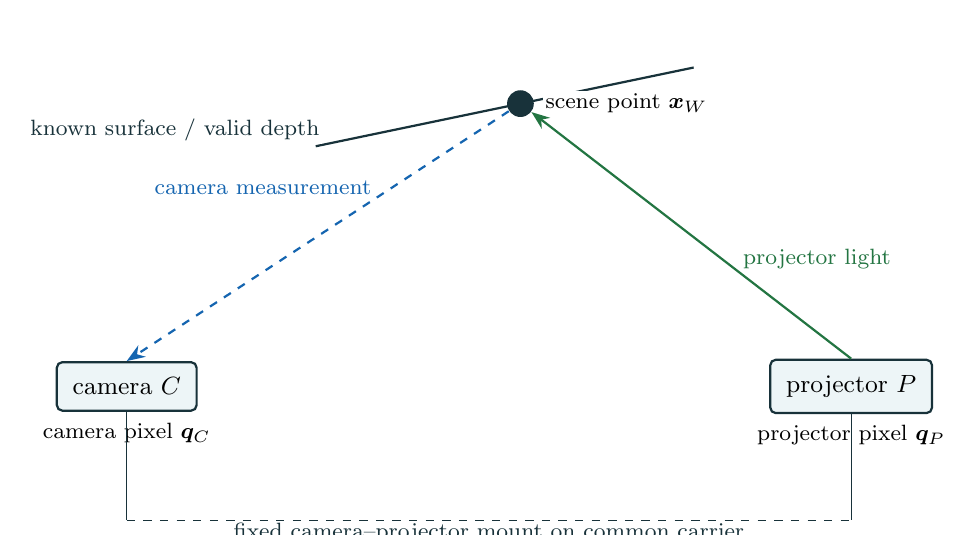
\begin{tikzpicture}
  % surface and shared point
  \draw[ink,thick] (-2.2,3.05) -- (2.6,4.05)
    node[flab,above left,pos=0.02]{known surface / valid depth};
  \node[circle,fill=ink,inner sep=1.2mm] (X) at (0.4,3.5916667) {};
  \node[flab,right=1mm of X] {scene point $\pt{W}$};
  % devices
  \node[flow] (C) at (-4.6,0) {camera $C$};
  \node[flow] (P) at (4.6,0) {projector $P$};
  \node[flab,below=1mm of C] {camera pixel $\bm{q}_C$};
  \node[flab,below=1mm of P] {projector pixel $\bm{q}_P$};
  % rays
  \draw[dedge,IO] (X) -- node[flab,text=IO,pos=0.35,above left]
    {camera measurement} (C.north);
  \draw[edge,VIS] (P.north) -- node[flab,text=VIS,pos=0.35,above right]
    {projector light} (X);
  % mount baseline
  \draw[ink,dashed] (-4.6,-1.7) -- node[flab,below]
    {fixed camera--projector mount on common carrier} (4.6,-1.7);
  \draw[ink] (C.south) -- (-4.6,-1.7) (P.south) -- (4.6,-1.7);
\end{tikzpicture}
\captionof{figure}{A camera pixel identifies a ray, not a unique 3D
point. A known surface or valid depth supplies the missing location. The
projector must illuminate that same point from its different lens center,
so camera and projector pixels generally differ. This sketch is not to
scale.}
\label{fig:camera-projector-rays}
\end{minipage}
\end{center}

\subsection{Depth is an additional measurement, not a replacement for pose}
If a depth image reports \emph{axial depth} $z_D$ in metres at an undistorted
depth pixel, then
\begin{equation}
\pt{D}=z_D(x_n,y_n,1)^\top,\qquad
\hpt{C}=\T{C}{D}\hpt{D},\qquad
\hpt{W}=\T{W}{D}(t)\hpt{D}.
\end{equation}
If the sensor instead reports radial range $\ell$, use
$\pt{D}=\ell\,\bm{d}_D/\|\bm{d}_D\|$.
Depth and color have distinct intrinsics, distortion and image sizes.
Use the measured color/depth transform and temporal registration;
holes, multipath, reflective surfaces and occlusion remain.

\textbf{Example 4.} At pixel $(20,10)$ with the tiny $K$,
axial depth $2$ m produces $\pt{D}=(0.5,0.25,2)$ m.
If the reported value were radial range $2$ m, the result would instead be
$2(0.25,0.125,1)/\sqrt{1.078125}$ m.

\subsection{Exactly when a homography is enough}
In an undistorted pinhole model, for a plane whose \emph{world coordinates}
are $(X,Y,0)$, let $\bm{r}_1,\bm{r}_2$ be the first two columns of
$\Rot{P}{W}$ and $\bm{t}=\tr{P}{W}$.
The planar map is
\begin{equation}
\bar{\bm{q}}_P\sim
H_P(X,Y,1)^\top,\qquad
H_P=K_P[\bm{r}_1\ \bm{r}_2\ \bm{t}].
\end{equation}
The symbol $\sim$ means equality up to nonzero scale, followed by division
by the third component. For two devices seeing that plane,
$H_{P\leftarrow C}=H_PH_C^{-1}$, when $H_C$ is invertible.
Nonzero lens distortion needs explicit undistortion/redistortion around
the homography. A table plane, a raised FF top, and its sloping faces are
different planes.

For a general mesh, render from each projector's own calibrated view,
using its current pose and lens warp. If the physical surface itself moves,
predict its pose as well as the projector's.
Anamorphosis additionally depends on a selected viewer-eye pose; a viewer
camera is not automatically the projector camera.

\subsection{Light overlap is radiometry, not just geometry}
At a surface point, let $g_j$ be projector $j$'s measured linear
irradiance-per-command gain (including distance, angle and reflectance),
and $a_j\in[0,1]$ its linear-light command. With ambient contribution
$E_{\rm amb}$,
\begin{equation}
E=E_{\rm amb}+\sum_j g_ja_j .
\label{eq:light}
\end{equation}
For desired added light $E_\star$ and nonnegative spatial weights
$w_j$ summing to one over available projectors, one simple allocation is
$a_j=\operatorname{clip}(w_jE_\star/g_j,0,1)$ for $g_j>0$.
Clipping means the target may be unattainable. Apply measured transfer
functions for display gamma/color; black levels cannot cancel ambient light.
A blanket ``each node uses $1/n$ brightness'' works only for equal calibrated
gains and actual overlapping coverage. Modifying LED current requires a
supported hardware interface, not an assumed HDMI feature.

Smoke/haze permits visible beams, not arbitrary opaque 3D surfaces.
Keep the beam-sculpture mode separate from the surface-mapping mode and
use venue-approved haze, ventilation and accessible alternatives.

\section{Time: Calibrate When the Light Lands, Not When a Packet Arrives}
\label{sec:time}

\begin{plain}{There are two kinds of lateness}
A frame can be geometrically accurate for a carrier pose from 60 ms ago.
That does not make it accurate for the moving carrier now.
Making a renderer run smoothly addresses cadence; measuring and predicting
to the light-emission time addresses age. These are different problems.
\end{plain}

\subsection{Timestamps and clock alignment}
For one frame, define capture/exposure midpoint $t_c$, tracking completion
$t_s$, render sampling time $t_r$, and intended light-emission time $t_\ell$.
End-to-end age is
\begin{equation}
\tau=t_\ell-t_c
=\tau_{\rm readout}+\tau_{\rm queue}+\tau_{\rm solve}
 +\tau_{\rm transport}+\tau_{\rm render}
 +\tau_{\rm present/display}.
\label{eq:latency}
\end{equation}
These terms must be measured without double-counting overlapping stages.
Include exposure integration, rolling shutter and display scanout in the
timing model where relevant. A global shutter avoids row-dependent
exposure poses but not exposure blur or downstream buffering.
Application-submit time is not camera exposure time.

Device monotonic clock $t_d$ maps approximately to session clock $t_W$ by
\begin{equation}
t_W=a_dt_d+b_d .
\end{equation}
Here $a_d$ is clock rate/skew and $b_d$ offset; estimate them over time and
publish uncertainty. Arrival time includes network delay.
As a simple offset probe, client send/receive times $t_1,t_4$ and server
receive/send times $t_2,t_3$ give
$\hat b=((t_2-t_1)+(t_3-t_4))/2$ and round-trip network estimate
$(t_4-t_1)-(t_3-t_2)$, \emph{assuming approximately symmetric delays and
negligible drift during the probe}. Asymmetry creates offset error.
Do not subtract different computers' raw monotonic clocks.

\subsection{Interpolation is behind; prediction is ahead}
For known body-to-world poses at $t_0<t_1$ bracketing a desired time $t$,
write their centers $\bm{c}_0,\bm{c}_1$ and rotations $R_0,R_1$.
Let $\alpha=(t-t_0)/(t_1-t_0)$, with $0\leq\alpha\leq1$:
\begin{equation}
\bm{c}(t)=(1-\alpha)\bm{c}_0+\alpha\bm{c}_1,\qquad
R(t)=R_0\Exp\!\left(\alpha\Log(R_0^\top R_1)\right).
\label{eq:interp}
\end{equation}
$\Exp$ maps a three-component rotation vector to a rotation matrix
(Rodrigues); $\Log$ maps a relative rotation to its principal rotation
vector. Quaternion SLERP is another way to perform this orientation
interpolation with appropriate sign/shortest-path handling.
Do not call SLERP directly on a $4\times4$ matrix.

For display time \emph{after} the latest measurement, use a model.
With world linear velocity $\bm{v}$, body angular velocity $\bm{\omega}$
and horizon $h=t_\ell-t_k\geq0$,
\begin{equation}
\hat{\bm{c}}(t_\ell)=\hat{\bm{c}}_k+\hat{\bm{v}}_kh,\qquad
\hat R(t_\ell)=\hat R_k\Exp(\hat{\bm{\omega}}_kh).
\label{eq:predict}
\end{equation}
This is constant-velocity extrapolation, not a guarantee. Cap horizon and
uncertainty; it cannot anticipate an unexpected impact or carrier slew.
Measure velocity in the stated frame, not by differencing unrelated
world-to-camera translation vectors.

If the surface is FF-attached and both surface and projector move, evaluate
\begin{equation}
\T{P}{F}(t_\ell)=
\T{W}{P}(t_\ell)^{-1}\T{W}{F}(t_\ell).
\end{equation}
Predicting only one side still produces a temporal mismatch.
An optional neural predictor must earn its place against these baselines
on held-out motion, report uncertainty, and fall back safely.
Neither an NPU nor adaptive process noise creates missing geometric evidence.
Figure~\ref{fig:capture-to-light} shows the two timelines involved.

\begin{center}
\begin{minipage}{\linewidth}
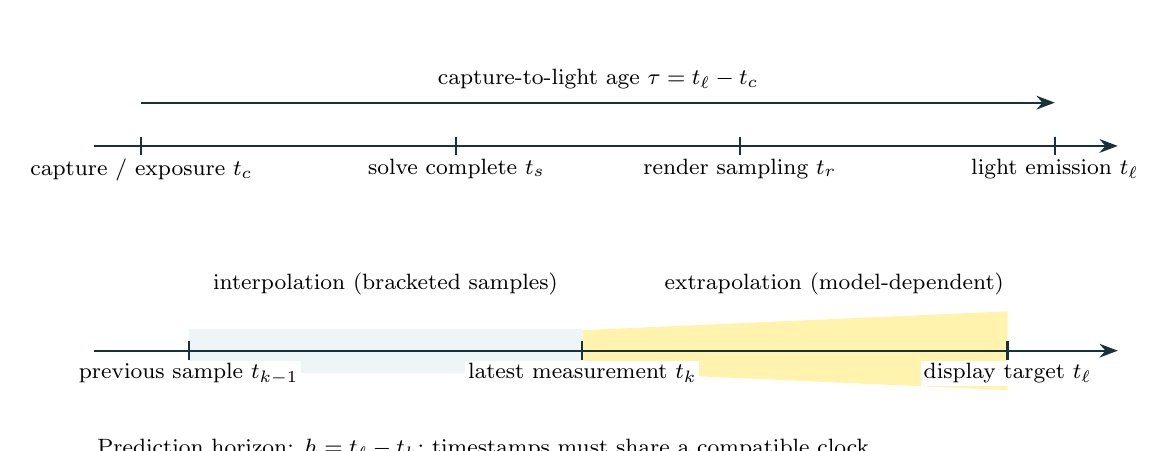
\begin{tikzpicture}
  % top band: pipeline clocks
  \draw[ink,thick,-{Stealth}] (0,0) -- (13,0);
  \foreach \x/\t in {0.6/{capture / exposure $t_c$},
    4.6/{solve complete $t_s$}, 8.2/{render sampling $t_r$},
    12.2/{light emission $t_\ell$}}{
    \draw[ink,thick] (\x,0.12) -- (\x,-0.12);
    \node[flab,below] at (\x,-0.12) {\t};}
  \draw[edge] (0.6,0.55) -- (12.2,0.55);
  \node[flab] at (6.4,0.85) {capture-to-light age $\tau=t_\ell-t_c$};
  % bottom band: samples vs target
  \fill[paperblue] (1.2,-2.32) rectangle (6.2,-2.88);
  \fill[APPfill] (6.2,-2.34) -- (11.6,-2.1) -- (11.6,-3.1)
    -- (6.2,-2.86) -- cycle;
  \draw[ink,thick,-{Stealth}] (0,-2.6) -- (13,-2.6);
  \draw[ink,thick] (1.2,-2.48) -- (1.2,-2.72);
  \draw[ink,thick] (6.2,-2.48) -- (6.2,-2.72);
  \draw[ink,thick] (11.6,-2.48) -- (11.6,-2.72);
  \node[flab,below] at (1.2,-2.72) {previous sample $t_{k-1}$};
  \node[flab,below] at (6.2,-2.72) {latest measurement $t_k$};
  \node[flab,below] at (11.6,-2.72) {display target $t_\ell$};
  \node[flab] at (3.7,-1.75) {interpolation (bracketed samples)};
  \node[flab] at (9.4,-1.75) {extrapolation (model-dependent)};
  \node[flab,anchor=west] at (0,-3.85)
    {Prediction horizon: $h=t_\ell-t_k$; timestamps must share a
     compatible clock.};
\end{tikzpicture}
\captionof{figure}{Smooth frame cadence does not remove the age of the
observations. Interpolation uses bracketing samples; beyond the latest
measurement, display-time pose is a prediction with uncertainty. Camera,
joint and display timing must use a compatible clock. Timeline spacing
and uncertainty shading are schematic, not measurements.}
\label{fig:capture-to-light}
\end{minipage}
\end{center}

\subsection{Example 5: Smooth does not mean aligned}
A lantern's optical carrier slews at $90^\circ$/s with 60 ms
capture-to-light age; the gimbal can rotate the carrier even while the
handle stays still.
It turns $5.4^\circ$ during that delay. At a 2 m perpendicular surface,
the uncompensated angular displacement is about
$2\tan(5.4^\circ)=0.1891$ m.
Even a 1 ms clock error at that speed contributes approximately 3.14 mm
at 2 m. This is why ``millimetre precision'' must state motion and timing.

\section{Tracking, IMUs, Dropouts, and Recovery}
\label{sec:tracking}

\subsection{A visual-only filter and a visual--inertial filter are not the same}
The repository's pose EKF smooths visual poses with estimated linear and
angular velocity. That is useful; it is not evidence of IMU fusion.
For a proposed body IMU, a suitable nominal state is
\begin{equation}
\bm{x}=(\bm{c},\bm{v},R,\bm{b}_a,\bm{b}_g).
\end{equation}
Here $\bm{c}$ is body origin in $W$, $\bm{v}$ world velocity,
$R=\Rot{W}{B}$, and $\bm{b}_a,\bm{b}_g$ are three-component accelerometer
and gyroscope biases. Align the IMU axes and lever arm to $B$ first.
For simplicity this model places the body origin at the IMU; use the fixed
camera/IMU offset when converting a visual observation to this origin.

Let measured specific force be $\bm{a}_m$, measured angular rate
$\bm{\omega}_m$, and gravity $\bm{g}=(0,0,-9.81)^\top$ m/s$^2$ in a
$z$-up room. Over a short step $\Delta t$,
\begin{align}
\bm{a}_W&=R(\bm{a}_m-\bm{b}_a)+\bm{g},\\
\bm{c}^-&=\bm{c}+\bm{v}\Delta t+\tfrac12\bm{a}_W\Delta t^2,\\
\bm{v}^-&=\bm{v}+\bm{a}_W\Delta t,\\
R^-&=R\Exp((\bm{\omega}_m-\bm{b}_g)\Delta t).
\label{eq:imu}
\end{align}
Biases are approximately constant over this step with random-walk noise.
At rest, specific force balances gravity after rotation.
Accelerometer bias accumulates position error; a magnetometer near stage
metal/electronics is not a reliable absolute yaw guarantee.
An IMU does not maintain drift-free position through arbitrary occlusion.

\subsection{The uncertainty update, with rotations treated correctly}
Use a 15-component local error
$\delta\bm{x}=(\delta\bm{c},\delta\bm{v},\delta\bm{\theta},
\delta\bm{b}_a,\delta\bm{b}_g)$.
Orientation error is defined on the right:
$R_{\rm true}\simeq R\Exp(\delta\bm{\theta})$.
Write corrected IMU samples as
$\bm{a}=\bm{a}_m-\bm{b}_a$, $\bm{\omega}=\bm{\omega}_m-\bm{b}_g$.
The first-order continuous error Jacobian $F_c$ is
\begin{equation}
F_c=\begin{bmatrix}
0&I&0&0&0\\
0&0&-R\sk{\bm{a}}&-R&0\\
0&0&-\sk{\bm{\omega}}&0&-I\\
0&0&0&0&0\\
0&0&0&0&0
\end{bmatrix},\quad
F\simeq I+F_c\Delta t,\quad
P^-=FPF^\top+Q_d.
\end{equation}
Each block is $3\times3$; $Q_d$ is discrete process-noise covariance,
obtained by integrating rotated accelerometer/gyro noise and bias random
walks over the step. Tune from sensor characterization, not visual
preference; use finer integration for rapid motion.

For frozen Jacobians over a short step, let $Q_c$ be the $12\times12$
continuous spectral-density matrix of independent accelerometer noise,
gyro noise, accelerometer-bias walk and gyro-bias walk (three components
each). Their error-state injection matrix and discretization are
\begin{equation}
\mathcal G=\begin{bmatrix}
0&0&0&0\\-R&0&0&0\\0&-I&0&0\\0&0&I&0\\0&0&0&I
\end{bmatrix},\qquad
Q_d=\int_0^{\Delta t}\Phi(s)\mathcal G Q_c\mathcal G^\top\Phi(s)^\top\,ds,
\quad \Phi(s)=e^{F_cs}.
\end{equation}
Each block in $\mathcal G$ is $3\times3$; $Q_c$ must use consistent SI
units. A first-order approximation is
$Q_d\simeq\mathcal G Q_c\mathcal G^\top\Delta t$ when sufficiently small
time steps justify it.

Convert visual PnP through Equations~\eqref{eq:movingcam} and
\eqref{eq:body} into a body pose measurement
$(\bm{c}_z,R_z)$ \emph{at exposure time}.
Transform its covariance into the same world-position/body-angle convention.
Let $N$ be its $6\times6$ covariance including relevant anchor uncertainty.
The innovation $\bm{r}$, observation Jacobian $H$, innovation covariance
$S$, and gain $L$ are
\begin{align}
\bm{r}&=\begin{bmatrix}
\bm{c}_z-\bm{c}^-\\ \Log((R^-)^\top R_z)
\end{bmatrix},&
H&=\begin{bmatrix}I&0&0&0&0\\0&0&I&0&0\end{bmatrix},\\
S&=HP^-H^\top+N,&
L&=P^-H^\top S^{-1},\qquad
\delta\hat{\bm{x}}=L\bm{r}.
\end{align}
Gate outliers using $\bm{r}^\top S^{-1}\bm{r}$ and independent geometric
checks; a probability-based threshold requires a justified noise model.
Apply position, velocity and bias corrections additively; apply
$R^+=R^-\Exp(\delta\hat{\bm{\theta}})$.
Before resetting the local error to zero, use the Joseph covariance update
and first-order orientation reset Jacobian:
\begin{align}
\widetilde P&=(I-LH)P^-(I-LH)^\top+LNL^\top,\\
J_{\rm reset}&=\operatorname{diag}
(I,I,I-\tfrac12\sk{\delta\hat{\bm{\theta}}},I,I),&
P^+&=J_{\rm reset}\widetilde P J_{\rm reset}^\top.
\end{align}
This derivation is a first-order local error-state model, not a ready-made
global VIO implementation. Large inconsistent rotations should trigger
validated relocalization rather than a tiny-angle correction.

For a delayed visual result, correct a stored state at its exposure time and
replay the intervening IMU samples. Applying an old image as if captured
now produces a biased state. Predicted/filtered samples from the same
measurements are correlated: do not fuse them as independent sensors.

\subsection{An explicit live state machine}
\begin{tabularx}{\linewidth}{@{}L{26mm}XX@{}}
\toprule
State & Evidence & Rendering policy\\ \midrule
Unregistered & No valid world alignment & Setup/status only; no room-locked light\\
Tracking & Fresh accepted pose and valid calibration & Render at estimated display time\\
Weak & Small/planar marker, poor coverage, uncertain map & Broader/less sensitive visuals; show quality\\
Coasting & No new accepted fix; bounded model prediction & Short, uncertainty-limited continuation\\
Lost & Age, uncertainty or motion budget exceeded & Fade/blank spatial output; preserve artwork data\\
Relocalizing & New plausible absolute observations & Validate before accepting a new world pose\\
Relative-only & Relative tracking survives, world link lost & Optional explicitly labelled object-locked mode\\
\bottomrule
\end{tabularx}

A known static projector can keep rendering room-locked artwork during a
camera dropout if its pose and the surface remain trusted.
A moving projector must not simply freeze its last image and call that
world-lock. For a carried lantern, rapid carrier or handle motion or
uncertain pose should cause earlier blanking. These are alignment policies, not optical certification.
Figure~\ref{fig:tracking-recovery} summarizes the recovery loop.

\begin{center}
\begin{minipage}{\linewidth}
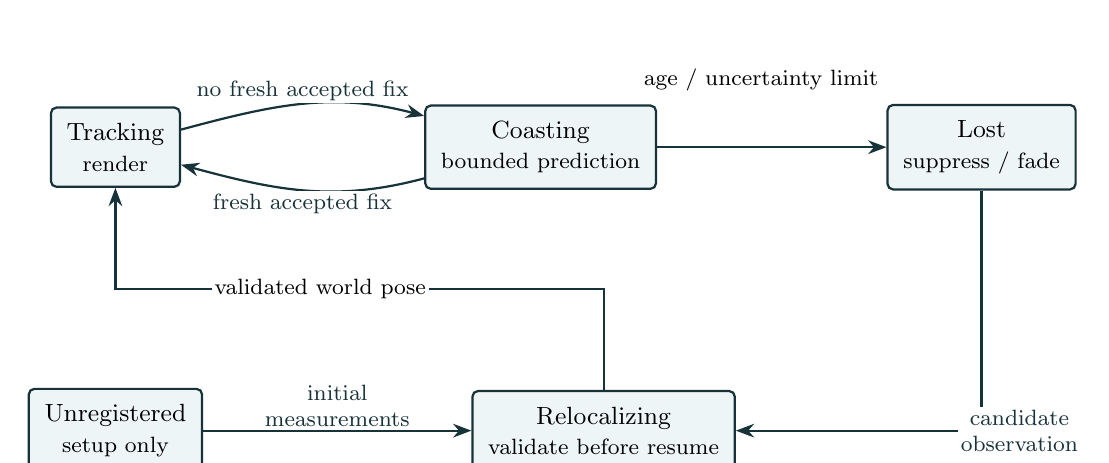
\begin{tikzpicture}
  \node[flow] (trk) at (0,0) {Tracking\\ \footnotesize render};
  \node[flow] (cst) at (5.4,0) {Coasting\\ \footnotesize bounded prediction};
  \node[flow] (lost) at (11.0,0) {Lost\\ \footnotesize suppress / fade};
  \node[flow] (unr) at (0,-3.6) {Unregistered\\ \footnotesize setup only};
  \node[flow] (rel) at (6.2,-3.6) {Relocalizing\\ \footnotesize validate before resume};
  \draw[edge] (trk) to[out=15,in=165]
    node[flab,above]{no fresh accepted fix} (cst);
  \draw[edge] (cst) to[out=195,in=-15]
    node[flab,below]{fresh accepted fix} (trk);
  \draw[edge] (cst) -- (lost);
  \node[flab] at (8.2,0.85) {age / uncertainty limit};
  \draw[edge] (lost.south) |- node[flab,pos=0.55,right]
    {candidate\\ observation} (rel.east);
  \draw[edge] (rel.north) -- (6.2,-1.8) -- (0,-1.8) -- (trk.south);
  \node[flab] at (2.6,-1.8) {validated world pose};
  \draw[edge] (unr) -- node[flab,above]{initial\\ measurements} (rel);
\end{tikzpicture}
\captionof{figure}{Simplified recovery loop: losing a pose does not
delete the canvas. The full state table also covers Weak and
Relative-only operation; neither creates missing room-reference
evidence. Homing or controller faults can independently suppress
projection even when a geometric pose is available.}
\label{fig:tracking-recovery}
\end{minipage}
\end{center}

\textbf{Recovery after a long loss.} Detect full-frame; solve multiple
candidates where appropriate; check positive depth and model consistency;
validate against fixed landmarks or an independent tracker; require a stable
sequence according to the installation's tested acceptance policy.
Reset or reinitialize the estimator if the old prediction is inconsistent.
Keep canvas coordinates fixed. A cosmetic fade can hide a pose correction,
but smoothing must not make a known wrong calibration appear valid.

\textbf{Bumps.} Compare observed fixed-landmark corners with predictions from
the stored fixed-camera pose. A fresh PnP fit may have a low residual
after a bump, so monitoring only its post-fit residual misses the event.
Separate camera displacement, FF motion, bad correspondences, and lens changes
using independent constraints. Update only affected transforms.

\section{Collaborative Canvas and the Spatial Pipe}
\label{sec:pipe}

\begin{plain}{Share the score, not everyone's screen recording}
Transmit strokes, attachments, transforms and show events.
Each capable node renders locally from its own current pose.
This keeps carrier motion off the Wi-Fi critical path.
The network still matters for agreement, ordering, authentication and
shared calibration; it does not replace local sensing.
\end{plain}

\subsection{Choose a practical first topology}
Use one session coordinator for identity, authoritative calibration revisions,
content event order, and discovery. Keep tracking and projection local.
On coordinator loss, already registered nodes may continue trusted local
rendering and buffer artwork events, but cannot invent conflicting new
world epochs. A router is not necessarily an application server.

This is \textbf{distributed rendering with coordinated session state}, not a
claim of fully decentralized consensus. MQTT normally involves a broker;
WebSockets supply transport, not discovery or peer consensus. A later peer
system must define leader election, partitions and merge rules explicitly.

\subsection{Artwork must declare what it is attached to}
For a stroke vertex $\hpt{A}$ stored in attachment frame $A$,
\begin{equation}
\hpt{W}(t)=\T{W}{A}(t)\hpt{A},\qquad
\bm{q}_{P}(t)=
\pi_P\!\left(\T{P}{W}(t)\T{W}{A}(t)\hpt{A}\right).
\label{eq:canvas}
\end{equation}
Choose $A=W$ for room-lock, $A=F$ for FF-lock, or a tracked object.
Store samples at their creation time and in their declared attachment,
not in the current producer-camera frame.

A stroke created in $F$ at $t_0$ and then baked into the room uses
$\hpt{W}=\T{W}{F}(t_0)\hpt{F}$ forever.
A genuinely FF-attached stroke instead uses $\T{W}{F}(t)$ every frame.
This one decision determines whether the artwork follows the prop.
Figure~\ref{fig:canvas-attachments} shows both behaviors on one ruler.

\begin{center}
\begin{minipage}{\linewidth}
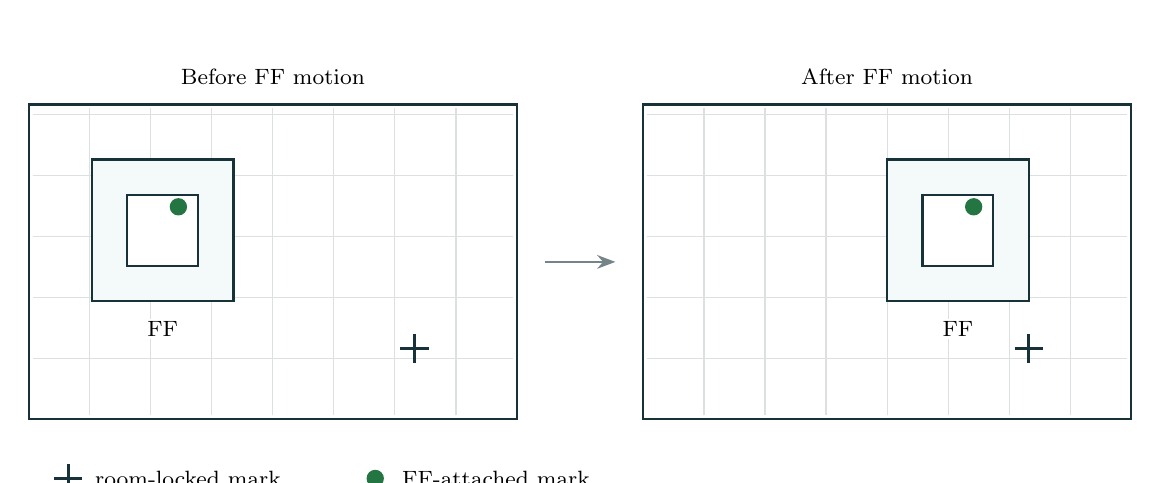
\begin{tikzpicture}
  % ---- panel 1: before (local coordinates) ----
  \draw[ink,thick,fill=white] (0,0) rectangle (6.2,4.0);
  \draw[ink!15,step=0.775] (0.05,0.05) grid (6.15,3.95);
  \node[flab] at (3.1,4.35) {Before FF motion};
  \draw[ink,thick,fill=paperblue!60] (0.8,1.5) rectangle (2.6,3.3);
  \draw[ink,thick,fill=white] (1.25,1.95) rectangle (2.15,2.85);
  \node[flab] at (1.7,1.15) {FF};
  \fill[VIS] (1.9,2.7) circle (0.11);
  \draw[ink,line width=1pt] (4.72,0.9) -- (5.08,0.9) (4.9,0.72) -- (4.9,1.08);
  % transition arrow
  \draw[-{Stealth},thick,ink!60] (6.55,2.0) -- (7.45,2.0);
  % ---- panel 2: same local coordinates, shifted scope ----
  \begin{scope}[shift={(7.8,0)}]
    \draw[ink,thick,fill=white] (0,0) rectangle (6.2,4.0);
    \draw[ink!15,step=0.775] (0.05,0.05) grid (6.15,3.95);
    \node[flab] at (3.1,4.35) {After FF motion};
    % FF + attached mark: same local offset, shifted right by 2.3
    \draw[ink,thick,fill=paperblue!60] (3.1,1.5) rectangle (4.9,3.3);
    \draw[ink,thick,fill=white] (3.55,1.95) rectangle (4.45,2.85);
    \node[flab] at (4.0,1.15) {FF};
    \fill[VIS] (4.2,2.7) circle (0.11);
    % room mark at identical local coordinates
    \draw[ink,line width=1pt] (4.72,0.9) -- (5.08,0.9)
      (4.9,0.72) -- (4.9,1.08);
  \end{scope}
  % legend
  \draw[ink,line width=1pt] (0.32,-0.75) -- (0.68,-0.75)
    (0.5,-0.93) -- (0.5,-0.57);
  \node[flab,anchor=west] at (0.8,-0.75) {room-locked mark};
  \fill[VIS] (4.4,-0.75) circle (0.11);
  \node[flab,anchor=west] at (4.7,-0.75) {FF-attached mark};
\end{tikzpicture}
\captionof{figure}{Room-locked marks stay fixed when the FF moves.
FF-attached marks keep their local coordinates and move with it. Moving a
lantern changes the rendering viewpoint, not either mark's attachment.
The two panels use the same room ruler.}
\label{fig:canvas-attachments}
\end{minipage}
\end{center}

If a deliberate coordinate rebase creates a new room epoch $W'$ with
$G=\T{W'}{W}$, transform \emph{all} room-locked geometry and world poses
consistently, e.g.
$\hpt{W'}=G\hpt{W}$ and $\T{W'}{B}=G\T{W}{B}$.
Do not overwrite the origin silently while leaving old strokes untouched.
A map correction and a coordinate rebase are different operations.

\subsection{A concrete, proposed message contract}
The following is a \textbf{new protocol specification}, not the current
\texttt{fulcrum\_poses.json} schema. Matrix rows are row-major serialized
arrays but multiply column vectors as in Equation~\eqref{eq:transform}.
The pose covariance uses order $(\delta c_x,\delta c_y,\delta c_z,
\delta\theta_x,\delta\theta_y,\delta\theta_z)$, world translation/right-local
rotation convention.
\begin{lstlisting}
{
  "schema": "shared-light.pose/1",
  "session_id": "gallery-session",
  "world_epoch": 3,
  "calibration_revision": "rig-r17",
  "geometry_revision": "ff-v1-survey-02",
  "device_id": "lantern-a",
  "sequence": 1842,
  "from_frame": "optical-carrier:lantern-a",
  "to_frame": "world:3",
  "units": "m",
  "clock_id": "session-monotonic",
  "capture_time_s": 12.400,
  "estimate_time_s": 12.400,
  "valid_until_s": 12.430,
  "clock_sigma_s": 0.001,
  "T_to_from": [[1,0,0,0.4], [0,1,0,0.2],
                [0,0,1,1.5], [0,0,0,1]],
  "status": "tracking",
  "evidence_ids": ["cam-a:frame-442"],
  "covariance_order": ["cx","cy","cz","rx","ry","rz"],
  "covariance_diagonal": [0.000025,0.000025,0.0001,
                          0.0001,0.0001,0.0004]
}
\end{lstlisting}
Numbers are illustrative, not measurements. The example only serializes a
diagonal covariance; a production full matrix must explicitly declare its
layout. A predicted estimate must have its own estimate time and keep the
original capture time. \texttt{valid\_until} is a policy budget, not proof of
future accuracy. Track measurement provenance to avoid double-counting
the same observation across relays.

Use separate message families:
\begin{itemize}
  \item \textbf{Calibration snapshots:} reliable, retained, versioned and
    acknowledged; intrinsics, image processing, rigid offsets, marker map,
    clock conventions and validation report.
  \item \textbf{Pose telemetry:} latest valid state wins; sequence checks,
    timestamps, expiry, uncertainty, evidence provenance.
  \item \textbf{Artwork events:} reliable begin/append/end operations with
    stroke ID, author, attachment, sample times, local sequence and style.
  \item \textbf{Show commands:} authenticated mode changes scheduled in
    session time, with acknowledgements and an expiry/late policy.
\end{itemize}
For a first version, each stroke has one writer; append indices make retries
idempotent. A session event order resolves deletes and style changes;
tombstones prevent deleted strokes reappearing after reconnect.
Buffer offline edits with unique IDs and reconcile explicitly. Pose loss
must not delete the shared canvas.

\subsection{Queues, integration and access control}
Bound queues and discard superseded camera frames rather than process an
ever-older FIFO. Keep exposure timestamps through capture, tracking and
rendering. A larger queue can improve throughput statistics while worsening
interactive alignment.

Use worker processes/native code for heavy vision; Python threads alone do
not guarantee CPU parallelism. Keep TouchDesigner operator access on its
supported main-thread path. Exchange bounded immutable pose/image snapshots;
shared memory may still involve copies. Network OSC is not zero-copy memory.
Monitor tracking cadence, render cadence, GPU deadlines, data age, queue
depth and rejected measurements separately.

The existing TD bridge can execute Python remotely. Keep it on localhost or
a trusted restricted network; do not expose it as a public audience API.
Use a small authenticated allow-listed control API for phones, role-based
permissions for calibration changes, and explicit consent for camera capture.
Do not broadcast raw video unless it is specifically needed and agreed.

\section{Initial and On-the-Go Calibration: Operational Recipes}
\label{sec:recipes}

\subsection{Initial survey: before the first performance}
Figure~\ref{fig:calibration-flow} summarizes the order.
\begin{enumerate}
  \item \tagHW\ \textbf{Make it mechanically and optically safe.}
    Use a rigid optical carrier on its gimbal mount, strain relief,
    ventilation, tested power rails, conservative optical output and an
    accessible stop. Bench-test before any handheld use.
  \item \tagIO\ \textbf{Inventory the exact streams.}
    Record lens, serial ID, image size, crop, stabilization, exposure
    timing, depth units and output mode. Lock changing optics/warps.
  \item \tagIO\ \textbf{Calibrate lenses and timing.}
    Use diverse calibration views and held-out tests. Fit depth/color
    registration, IMU alignment and clock offsets where those sensors exist.
  \item \tagHW\ \textbf{Survey the FF and static references.}
    Measure actual corners, reserve unique IDs, version the geometry, and
    provide fixed room references if the FF is allowed to move.
  \item \tagIO\ \textbf{Establish the room once.}
    Hold the FF fixed; choose $\T{W}{F}(t_0)$; solve camera poses with
    Equation~\eqref{eq:initial}; verify static-camera baselines.
  \item \tagIO\ \textbf{Calibrate every projector.}
    Capture coded patterns and physical surface points. Solve projector
    lens/pose parameters and rigid camera--projector offsets.
    For a lantern, fit the camera and projector on the shared carrier as
    one rigid pair.
  \item \tagIO\ \textbf{Unlock, sweep and validate the gimbal.}
    With the joints locked, complete the rigid lens and offset fits above.
    Then unlock and sweep the joints: the measured camera--projector
    offset must stay invariant while the housing--carrier relation
    changes. The direct Route A prototype needs no encoder. Before
    enabling Route B, calibrate the joint axes, pivots, signs and encoder
    zeros, and align the camera, encoder and tracker clocks. Validate
    hold/follow/home/transport-lock transitions and controller-fault
    suppression before the show.
  \item \tagVIS\ \textbf{Measure independent alignment.}
    Use test points not used for fitting, including multiple depths and
    image edges. Test moving devices, dropout, and camera bumps.
  \item \tagAPI\ \textbf{Publish one coherent snapshot.}
    Stage all device results, validate them, atomically activate one
    revision, and require node acknowledgement. Retain the last known-good
    revision and report partial failure without mixing old and new results.
  \item \tagAPP\ \textbf{Rehearse the performance state machine.}
    Show tracking/weak/lost states, confirm which artwork is room-locked
    or object-locked, rehearse blanking and recovery, then enable the show.
\end{enumerate}

\begin{center}
\begin{minipage}{\linewidth}
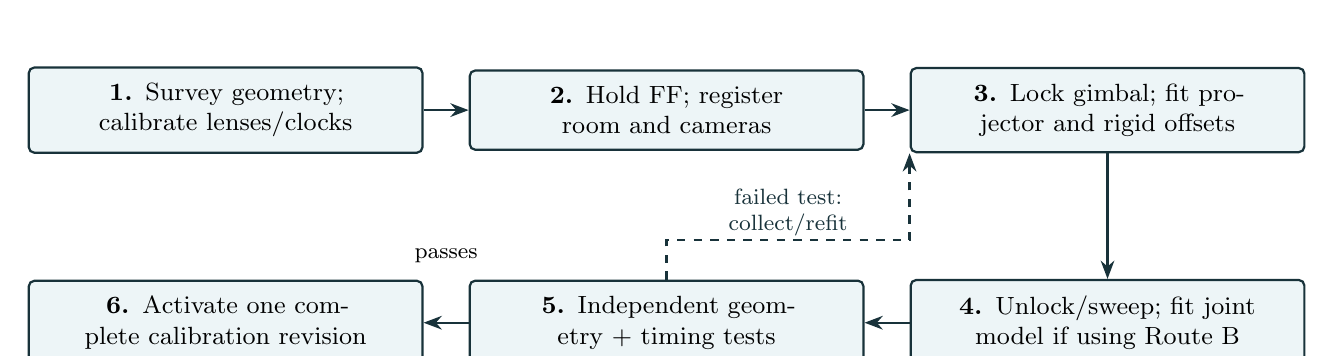
\begin{tikzpicture}
  \node[flow,text width=46mm] (b1) at (0,0)
    {\textbf{1.} Survey geometry; calibrate lenses/clocks};
  \node[flow,text width=46mm] (b2) at (5.6,0)
    {\textbf{2.} Hold FF; register room and cameras};
  \node[flow,text width=46mm] (b3) at (11.2,0)
    {\textbf{3.} Lock gimbal; fit projector and rigid offsets};
  \node[flow,text width=46mm] (b4) at (11.2,-2.7)
    {\textbf{4.} Unlock/sweep; fit joint model if using Route B};
  \node[flow,text width=46mm] (b5) at (5.6,-2.7)
    {\textbf{5.} Independent geometry + timing tests};
  \node[flow,text width=46mm] (b6) at (0,-2.7)
    {\textbf{6.} Activate one complete calibration revision};
  \draw[edge] (b1) -- (b2);
  \draw[edge] (b2) -- (b3);
  \draw[edge] (b3) -- (b4);
  \draw[edge] (b4) -- (b5);
  \draw[edge] (b5) -- (b6);
  \node[flab] at (2.8,-1.85) {passes};
  \draw[dedge] (b5.north) -- ++(0,0.5) -|
    node[flab,pos=0.25,above]{failed test:\\ collect/refit} (b3.south west);
\end{tikzpicture}
\captionof{figure}{Initial calibration produces a validated snapshot, not
a permanent promise. Revisit affected fits after optical or mechanical
changes. Routine lantern motion updates pose; it does not require a new
lens calibration each frame.}
\label{fig:calibration-flow}
\end{minipage}
\end{center}

\subsection{During a show: what to recalibrate, and when}
\begin{tabularx}{\linewidth}{@{}L{34mm}XX@{}}
\toprule Event & Correct operation & Do not do this\\ \midrule
FF moves, fixed reference remains & Update $\T{W}{F}(t)$; update
FF-attached content and device localization & Reset $W$ on every FF observation\\
Lantern carrier or housing moves & Track the optical carrier (directly, or
housing plus measured joints); predict to display time &
Refit lens distortion every frame\\
Static camera is bumped & Exclude its old world link; relocalize to fixed
landmarks or independently tracked FF & Infer camera motion from post-fit FF
residual alone\\
Static projector is bumped & Blank it; track its attached body or rerun
projected correspondences & Assume a separate static camera tracks its motion\\
Marker temporarily hidden & Bound prediction and uncertainty; fade as needed &
Keep calling stale pose ``tracked''\\
Gimbal homes, reaches a limit or faults & Suppress the affected projection;
check controller state and reacquire/validate the carrier pose before
resume & Treat motor commands or a homed flag as a measured pose\\
All room references lost & Relative mode or blackout; keep artwork stored &
Promise room-lock from IMU integration indefinitely\\
Focus/zoom/mount changes & Recheck lens or affected rigid calibration &
Treat mechanical changes as a software smoothing problem\\
New device joins & Load matching snapshot, calibrate its own lens and offsets,
localize and validate & Copy another device's $K$ or just scan an ID\\
\bottomrule
\end{tabularx}

\subsection{Python commands available in this repository today}
\label{sec:commands}
Run from the project root in a \textbf{Windows Command Prompt}.
The project CV interpreter is \texttt{C:\textbackslash Python314\textbackslash
python.exe}; the base Anaconda interpreter lacks the required CV modules.
These commands are documented here, \emph{not executed as part of writing
this document}. Calibration patterns alter live projector output and
require an attended, stationary setup.

\begin{lstlisting}
:: Existing offline rig solver: webcam + projector + Kinect by default.
:: Requires the running TD bridge and the expected FF network.
C:\Python314\python.exe tools\fulcrum\ff_calibrate.py

:: Explicitly omit Kinect registration:
C:\Python314\python.exe tools\fulcrum\ff_calibrate.py --no-kinect

:: Inspect CLI options without starting calibration:
C:\Python314\python.exe tools\fulcrum\ff_calibrate.py --help

:: Alternative standalone tracker; owns camera capture.
:: Do not run alongside TD capture for those same devices.
C:\Python314\python.exe tools\fulcrum\fulcrum_track.py
\end{lstlisting}
The old \texttt{--kinect} flag is not accepted by the current parser.
The default recalibrates the \emph{configured webcam/projector rig and
attempts Kinect registration}; it does not discover every camera on the
network or calibrate arbitrary lanterns.

\textbf{TD path, not the standalone path.}
\texttt{td\_ff\_live.py} is a TD module; its worker is
\texttt{ff\_worker.py}. Running the module as a normal standalone
Python CLI is not the supported live setup. Existing TD setup scripts can
build/modify the network and should only be used on the intended project.
The bridge's documented script invocation form is
\begin{lstlisting}
node tools/td/td.mjs --file <existing-setup-script.py>
\end{lstlisting}
The angle-bracket argument is a placeholder, not an executable command.
No general-purpose \texttt{xr calibrate-all}, mobile daemon, IMU fusion
service or gimbal control API is claimed to exist yet.

\subsection{Repository audit: current behavior versus the proposed system}
\label{sec:repoaudit}
This is a source inspection snapshot, not a live hardware diagnosis.
\begin{enumerate}
  \item \textbf{All-device publication is not transactional.}
    In \texttt{ff\_calibrate.py}, \texttt{main()} writes
    \texttt{calibration\_current.json} and calls \texttt{export\_viewer()}
    before \texttt{phase\_kinect()}. The export can therefore use the
    \emph{previous} Kinect registration. The archive is also written before
    that phase, and its \texttt{validated} field describes the earlier fit,
    not complete all-camera success. Kinect SDK import failure returns a skip.
    Default participation does not prove a coherent all-camera result.
  \item \textbf{The room anchor still depends on a frozen webcam pose.}
    \texttt{export\_viewer()} and \texttt{td\_ff\_live.py} use
    \texttt{aruco\_solve\_frozen.json} for the table/world link. Re-solving
    the FF alone does not refresh that independent link if the webcam moved.
    This is why rerunning one command is not an unconditional stale-anchor fix.
  \item \textbf{Fixed camera--projector links assume fixed hardware.}
    The live module constructs \texttt{projector\_from\_camera} from stored
    calibration and Kinect registration. That is appropriate for unchanged
    rig geometry, not independently moving devices.
  \item \textbf{The webcam fit is not a full lens calibration.}
    The offline solver refines a constrained pinhole model with priors and
    zero webcam distortion. Kinect K/D is fitted to factory mapper samples,
    not a fresh independent optical calibration of arbitrary cameras.
  \item \textbf{Worker isolation exists; a complete inertial pipe does not.}
    \texttt{ff\_worker.py} uses a separate process and shared-memory buffers
    with image copies. \texttt{pose\_ekf.py} is a visual pose/velocity filter;
    this inspected path does not implement the proposed 200 Hz IMU/NPU system.
    Live timestamps include application-level timing, not a demonstrated
    hardware exposure-to-photon synchronization system.
  \item \textbf{Hold/fade is a visual policy, not guaranteed tracking.}
    TD defaults include a 1.5 s hold/fade window and a 0.25 s filter
    reacquisition setting, subject to controls. This is not a measured
    safe carrier prediction horizon. The separate painted-solid tracker
    has different constants and is not the stage-scale FF document model.
\end{enumerate}
These are implementation tasks in Section~\ref{sec:tasks}; this document
does not silently modify the live rig.

\section{Joint Refinement and an Honest Validation Plan}
\label{sec:validation}

\subsection{A connected calibration graph}
Think of frames as nodes and measured transforms as edges.
Every device needing room-lock must have a valid, time-consistent path to
$W$. Fix the room frame (or one surveyed anchor pose) so the optimization
does not float. Metric surveyed geometry fixes scale; unconstrained
monocular mapping otherwise has a scale ambiguity.

Let $\Theta$ collect the unknown lens parameters, body/device offsets,
per-time poses and any explicitly estimated surface parameters.
For camera observation $i$ at time $t_i$ of a point stored on attachment
frame $A_i$, predict
\begin{equation}
\hat{\bm{q}}_i=
\pi_{C_i}\bigl(\T{C_i}{W}(t_i)\T{W}{A_i}(t_i)
\hpt{A_i,i}\bigr).
\end{equation}
Projector correspondences use the same expression with $P_j$ instead of
$C_i$. If axial depth observation $z_i$ is associated with an independently
specified corresponding world point $\pt{W,i}$, its residual is
\begin{equation}
e_i^D=z_i-\bm{e}_3^\top
\left(\Rot{D}{W}(t_i)\pt{W,i}+\tr{D}{W}(t_i)\right),
\qquad \bm{e}_3=(0,0,1)^\top.
\end{equation}
Do not back-project a depth sample with itself and call the resulting
zero depth residual an independent constraint. Surface correspondence,
registration, occlusion and noise must be modeled.

For visual/projector residual vectors $\bm{e}_i$ in pixels, depth errors
$e_i^D$ in metres, corresponding covariances $\Sigma_i$ and variances
$\sigma_{D,i}^2$, and explicit survey/rig priors $E_{\rm prior}$, a
dimensionally consistent joint objective is
\begin{equation}
\Theta^\star=\argmin_\Theta\left[
\sum_{i\in\mathcal V}\rho(\bm{e}_i^\top\Sigma_i^{-1}\bm{e}_i)
+\sum_{i\in\mathcal D}\rho((e_i^D)^2/\sigma_{D,i}^2)
+E_{\rm prior}(\Theta)\right].
\label{eq:bundle}
\end{equation}
$\mathcal V$ indexes image correspondences and $\mathcal D$ valid depth
constraints. Parameterize rotations with local increments.
With stacked whitened residual vector $\bm{r}(\Theta)$ and its Jacobian
$J$, a Levenberg--Marquardt step solves
$(J^\top J+\mu I)\Delta\Theta=-J^\top\bm{r}$, where $\mu>0$ is damping,
after appropriate parameter scaling and robust reweighting.
Convergence is not proof of correctness or sub-millimetre accuracy.
Use this offline or in a controlled background refinement, not as an
unbounded main-render-thread operation.

\subsection{Measure what an audience can actually see}
Define tolerances per installation, not one universal magic threshold.
Report at least:
\begin{itemize}
  \item \textbf{Static spatial accuracy:} independent projected test targets
    measured on physical surfaces, in mm, at several depths and viewing
    regions. Separate in-fit and held-out points.
  \item \textbf{Dynamic registration:} projected-target error while the rig
    moves through specified speeds/accelerations; report median, 95th
    percentile, maximum and failure counts with sample conditions.
  \item \textbf{Timing:} exposure-to-light latency and jitter, clock-offset
    uncertainty, tracking rate, render rate, rejected/dropped frames and
    pose age. Use independent timing evidence, such as a high-speed-camera
    or photodiode experiment with a defined stimulus.
  \item \textbf{Recovery:} duration and alignment error after FF occlusion,
    a bumped camera, moving prop, map reset, network loss and reconnect.
    Verify the world canvas does not jump or disappear.
  \item \textbf{Collaboration:} duplicate/reordered events, concurrent
    authors, deleted strokes, incompatible calibration revisions,
    unauthorized clients and coordinator restart.
  \item \textbf{Human/physical limits:} optical exposure assessment,
    enclosure temperature, runtime, mass balance, cable snag risks,
    accessibility and venue operating constraints.
\end{itemize}

For a near-normal planar surface at range $L$, small angular uncertainty
$\sigma_\theta$ contributes approximately $L\sigma_\theta$ displacement.
If independent small transverse translation uncertainty is $\sigma_c$,
an illustrative error budget is
$\sigma_{\rm hit}\simeq\sqrt{\sigma_c^2+(L\sigma_\theta)^2}$.
Add correlated calibration, surface and timing effects rather than treating
this approximation as an exact global bound.

\subsection{Power arithmetic without marketing units}
Battery energy is watt-hours (Wh), power is watts (W), and approximate
runtime is
\begin{equation}
t_{\rm run,h}\simeq\frac{\eta E_{\rm battery,Wh}}
 {P_{\rm compute}+P_{\rm projectors}+P_{\rm sensors}+P_{\rm gimbal}
  +P_{\rm cooling/network}} .
\end{equation}
$\eta$ is usable efficiency including conversion and reserve.
For an illustrative 74 Wh bank, $\eta=0.85$ and a \emph{measured} total
40 W load including motors, runtime would be about 1.57 h; this is not a
measurement of the proposed lantern. Capacity advertised in mAh needs its
reference voltage.

A 100 W bank may supply only 5 V/3 A on the port used by a Pi.
Verify the required profile, available current under simultaneous use,
fusing, and the gimbal's idle, slew and startup peaks, and thermal
behavior.
Raspberry Pi's official 27 W supply supports the relevant 5.1 V/5 A mode
\cite{pi-power}; a generic high-wattage label does not guarantee it.
The lantern housing carries the compute and battery below the gimbal, with
venting and an accessible power switch---there is no face-mounted design.
Do not assume long unshielded camera ribbons or joint-crossing cables will
work without signal-integrity tests.

\section{Build Plan: Color-Coded Tasks and Evidence of Done}
\label{sec:tasks}

\begin{tabularx}{\linewidth}{@{}lX@{}}
\tagHW & Hardware (red)\\
\tagIO & Input/output (blue)\\
\tagAPI & Pipe/network/integrations (purple)\\
\tagVIS & Visuals/animation (green)\\
\tagAPP & Applications (yellow)\\
\end{tabularx}

Tags and IDs remain legible in grayscale; yellow uses a pale fill with dark
gold text. Each task has one primary category; dependencies cross categories.
This is a proposed backlog, \textbf{not a list of completed features}.
``Done'' requires saved evidence, not just a plausible screenshot.

\subsection{Gate 0: Make a credible, safe bench rig}
\task{HW}{HW}{H1 / Survey and label the reference geometry}{
Measure FF corners and sticker offsets, record uncertainty and unique IDs;
separate desktop FF, painted solid and proposed stage structure.
\textbf{Done:} versioned survey and an independent dimension check.
\textbf{Feeds:} I1, I2.}
\task{HW}{HW}{H2 / Build the rigid optical carrier on its common gimbal}{
Mount the camera and projector together on one gimballed carrier;
balance the payload, keep joint clearances and lens apertures clear,
route cables with service loops, and provide a transport lock.
\textbf{Done:} the measured camera--projector offset stays invariant over
the full tested joint sweep and before/after independent handling.
\textbf{Feeds:} I3.}
\task{HW}{HW}{H3 / Verify electrical and thermal budgets}{
Test exact PD profiles, each rail, startup load, motor idle/slew/dynamic
loads, cabling, fuses, mass, enclosure temperature and sustained runtime.
\textbf{Done:} recorded load/temperature/runtime tests; no brownouts at
simultaneous maximum tested output.}
\task{HW}{HW}{H4 / Establish optical and mechanical operating safety}{
Exclude targeted blinding/IR countermeasures. Assess the complete projector
system under applicable optical standards and venue conditions; provide
accessible stop, conservative aiming, gimbal pinch-point guarding and
thermal/cable protections---a handheld beam can sweep bystanders.
IEC 62471-5 is relevant for image projectors, not a certification granted
by this document \cite{iec}.
\textbf{Done:} documented qualified assessment and operating envelope before
any handheld or gimballed audience trial.}
\task{IO}{I/O}{I1 / Inventory and calibrate each optical stream}{
Save exact K/D model, resolution, preprocessing, lens settings, depth units
and hardware identity. Acquire diverse intrinsic-calibration views.
\textbf{Done:} held-out residual maps and native/resized image consistency;
no shared master intrinsics. \textbf{Depends:} H1.}
\task{API}{API}{N1 / Define a versioned spatial contract}{
Specify transform direction, units, covariance convention, clocks, world
epoch, geometry revision, provenance, expiry and device IDs. Version the
carrier camera--projector offsets and, when Route B is used, the joint
model: axes, pivots, signs, encoder zeros and limits. These are
calibration snapshot metadata, not high-rate control telemetry.
\textbf{Done:} malformed, stale, wrong-unit and incompatible-revision
messages are rejected; synthetic transform round trips agree.
\textbf{Depends:} agreed conventions in Section~\ref{sec:notation}.}

\subsection{Gate 1: Prove static multi-device agreement}
\task{IO}{I/O}{I2 / Establish a room map with independent references}{
Register fixed cameras to surveyed static markers; register the FF without
making it the only live room reference.
\textbf{Done:} moving the FF leaves an independent room-locked test point
unchanged. \textbf{Depends:} H1, I1, N1.}
\task{IO}{I/O}{I3 / Calibrate each projector and rigid offset}{
Capture coded projected pixels on known surfaces, fit projector models,
and estimate camera/projector/carrier transforms on both devices.
\textbf{Done:} held-out alignment at multiple depths, with the fixed
internal camera--projector offset consistent across a joint sweep.
\textbf{Depends:} H2, I1, I2.}
\task{API}{API}{N2 / Fix all-device calibration publication}{
Stage webcam, projector and Kinect results before one atomic activation;
export viewer geometry from that same revision. Fail/report required
device skips, include the full outcome in the archive, and refresh an
invalid frozen room link rather than promising that FF-only fitting repairs it.
\textbf{Done:} an injected Kinect failure cannot publish a falsely complete
mixed revision; successful exports share the same revision.}
\task{VIS}{VIS}{V1 / Build the alignment and quality view}{
Draw predicted/detected corners, residual vectors, frame axes, projector
coverage, pose age, source IDs and tracking status. Distinguish raw,
filtered and predicted data.
\textbf{Done:} an intentionally wrong K, stale world link and wrong
baseline are visibly distinguishable. \textbf{Depends:} I2, I3, N1.}
\task{APP}{APP}{A1 / Ship a guided calibration application}{
Provide inventory, stationary-target instructions, captured evidence,
per-device pass/fail, snapshot review and last-good rollback.
\textbf{Done:} an unfamiliar operator completes the static setup without
editing matrices. \textbf{Depends:} N2, V1.}

\subsection{Gate 2: Move one light without moving the artwork}
\task{IO}{I/O}{I4 / Measure exposure-to-light timing}{
Preserve capture timestamps, characterize display buffering and clock
offset/skew, and align exposure, joint-encoder and display clocks across
static-camera and lantern captures.
\textbf{Done:} saved timing experiment and latency/jitter distributions,
with clock uncertainty. \textbf{Depends:} N1.}
\task{IO}{I/O}{I5 / Implement bounded live carrier tracking}{
Use direct optical-carrier relocalization (Route A) first; add calibrated
carrier-IMU propagation and delayed-state correction only when sensor
support exists. The housing-plus-encoder Route B additionally requires a
calibrated joint model and world-aligned housing tracking.
\textbf{Done:} tests for pose direction, gravity, biases, fast motion,
single-marker ambiguity, dropout and recovery on each enabled route;
Route B stays disabled until I6 and the independent housing--world link
are validated.
\textbf{Depends:} I2, I3, I4.}
\task{IO}{I/O}{I6 / Measure gimbal state and modes}{
Record measured joint angles and rates, zero/homing state, joint limits,
motor fault flags and per-sample timestamps. No encoder is required for
the direct visual-only Route A prototype; this task is required when using
the housing route or control supervision.
\textbf{Done:} slow and fast sweeps and handle-only movement distinguish
payload motion from housing motion; missing or stale joint samples
invalidate the housing-based route. \textbf{Depends:} H2, I4.}
\task{API}{API}{N3 / Separate capture, tracking and rendering deadlines}{
Keep bounded latest-frame queues, isolate CV work, retain timestamps and
make tracking age observable independently of render FPS.
\textbf{Done:} tracker slowdown increases reported age but does not grow an
unbounded FIFO or invoke unsupported TD operator work off-thread.
\textbf{Depends:} I4, N1.}
\task{VIS}{VIS}{V2 / Render the same surface from each current projector pose}{
Use calibrated per-projector views, distortion mapping, visibility/occlusion
and bounded display-time prediction of the carrier pose and surface.
Support static and moving projectors.
\textbf{Done:} moving one rig keeps an independent surface target aligned
within the declared dynamic tolerance. \textbf{Depends:} I3, I5, N3.}
\task{VIS}{VIS}{V3 / Make tracking failure legible and graceful}{
Implement tracking/weak/coasting/lost/relative-only states with tested
fade/blank behavior, suppression during untrusted slew, homing or
controller fault, and no silent coordinate reset.
\textbf{Done:} occlusion and bumps never label stale light as fully tracked.
\textbf{Depends:} I5, V1, V2.}
\task{APP}{APP}{A2 / Demonstrate room-lock versus prop-lock}{
Let an operator create one room-attached and one FF-attached mark, from a
carried housing and from gimbal-only carrier motion.
\textbf{Done:} moving the FF moves only the latter; moving the housing or
the carrier alone keeps room-locked artwork on its surface.
\textbf{Depends:} I2, V2, V3.}

\subsection{Gate 3: Share a canvas, not a calibration accident}
\task{API}{API}{N4 / Implement session discovery and authenticated control}{
Separate audience commands from the powerful TD execution bridge; restrict
calibration authority and support connection loss/rejoin.
\textbf{Done:} an unauthorized phone cannot execute Python or change the
world epoch. \textbf{Depends:} N1, A1.}
\task{API}{API}{N5 / Synchronize durable artwork and ephemeral poses}{
Use unique event IDs, single-writer strokes, append sequence numbers,
tombstones, snapshot recovery and latest-valid pose updates.
\textbf{Done:} duplication, reordering, partitions and reconnect do not
duplicate segments or resurrect deleted artwork.
\textbf{Depends:} N1, N4.}
\task{API}{API}{N6 / Integrate a bounded gimbal control interface}{
Separate commanded targets from measured joint state; publish controller
modes, limits, health, sequence numbers and sample age. Accept only
allowlisted authenticated commands with rate/position limits and a stop;
no arbitrary TD Python execution from a phone. This is a planned API, not
an existing CLI.
\textbf{Done:} stale or reordered telemetry is never treated as fresh
pose; a controller fault or homing sequence invokes the documented
projection suppression. \textbf{Depends:} N1, N4, I6.}
\task{VIS}{VIS}{V4 / Blend overlapping projectors in linear light}{
Measure gains, color/transfer response and overlap masks; account for
occlusion and unavailable emitters.
\textbf{Done:} an overlap test quantifies brightness/color differences and
clipping; a node leaving does not silently overdrive remaining units.
\textbf{Depends:} I3, V2, N5.}
\task{APP}{APP}{A3 / Build a collaborative surface-painting scene}{
Support author identity, brush styles, undo/delete, explicit attachments,
offline strokes and clear tracking status.
\textbf{Done:} two authors edit one persistent canvas and recover from a
network interruption without losing existing work.
\textbf{Depends:} A2, N5.}
\task{APP}{APP}{A4 / Add phone, Myo and mouse producers honestly}{
Use tracked phone rays; use Myo/sEMG for consented triggers and calibrated
orientation. Provide a declared fixed or tracked ray origin for IMU-only
tools; mouse unprojects through a chosen virtual view onto a chosen surface.
\textbf{Done:} the UI identifies each input's available degrees of freedom;
no orientation-only device claims absolute hand position.
\textbf{Depends:} A3, I5.}

\subsection{Gate 4: Portable lantern and artistic extensions}
\task{HW}{HW}{H5 / Package the portable lantern}{
Provide the vented housing with handle/stand, accessible controls,
serviceable joints and cable loops, payload and mass balance, and a
reproducible lock/unlock calibration check for transport.
\textbf{Done:} a carry/park/sweep/pack test preserves the measured
carrier calibration. \textbf{Depends:} H2--H4, I3--I5, V2.}
\task{VIS}{VIS}{V5 / Design visuals that tolerate measured uncertainty}{
Use larger features, surface-aware strokes, restrained animation and
deliberate transitions; label anamorphic single-view pieces and haze
beam sculptures as different modes.
\textbf{Done:} an artistic review and an error-overlay review agree about
which effects remain readable under the tested motion budget.
\textbf{Depends:} V3, V4.}
\task{APP}{APP}{A5 / Package rehearsal and performance modes}{
Provide consent, join/leave, venue setup, recording permissions, accessible
alternatives, show cues and an emergency stop. Store no raw sensor data by
default beyond the agreed diagnostic policy. Rehearse motor, cable and
power faults; no unattended gimbal sweeps around an audience.
\textbf{Done:} a rehearsal covers power/network/tracking/motor failure and
restart. \textbf{Depends:} H4, A1--A4, V3.}
\task{APP}{APP}{A6 / Treat neural prediction as a research experiment}{
Only after baseline measurement, compare classical prediction with any
learned model on held-out motion, including abrupt reversals.
\textbf{Done:} report error/latency distributions and failure behavior;
keep the simpler baseline if learning does not demonstrably improve it.
\textbf{Depends:} I4, I5, V2; optional, not a prerequisite for art.}

\section{Presentation Cheat Sheet}
\begin{tabularx}{\linewidth}{@{}L{36mm}X@{}}
\toprule Technical term & What to say out loud\\ \midrule
Intrinsic calibration & Learn the lens's pixel ruler and bending.\\
Extrinsic pose & Locate and orient a device relative to a named ruler.\\
PnP & Fit a known 3D shape to its measured image corners.\\
Shared world & Agree where the room ruler is, not just where packets go.\\
Rigid offset & Measure how the camera and light are bolted together.\\
Homography & A flat-surface shortcut, not a universal 3D warp.\\
Prediction & A short, uncertain guess about where things will be when light lands.\\
Spatial pipe & Exchange named, timed, versioned spatial facts and artwork.\\
Relocalization & Recover the room reference without moving the stored canvas.\\
Success & People move, collaborate and recover from errors without the light
pretending to know more than the sensors do.\\
\bottomrule
\end{tabularx}

\begin{plain}{The defensible project claim}
We are building a shared spatial canvas rendered by independent, calibrated
light sources. A measured reference object and additional persistent room
constraints connect local sensing to a common world. The system supports
both fixed and moving devices, explicitly manages timing and uncertainty,
and degrades visibly when evidence is missing.

That is a compelling artistic and computer-science project without claiming
zero latency, perfect tracking, or a free-floating hologram.
\end{plain}

\appendix
\section{Source Register and Traceability}
\label{sec:sources}
All nine Word documents were supplied from
\path{C:/Users/User/Downloads/ff_docs/drive-download-20261110T090728Z-1-001/}.
Their internal version numbers are document labels, not proof of completed
implementations.

\small
\begin{longtable}{@{}L{9mm}L{94mm}L{52mm}@{}}
\toprule Key & Exact supplied filename & Contribution / audit focus\\ \midrule
\endfirsthead
\toprule Key & Exact supplied filename & Contribution / audit focus\\ \midrule
\endhead
\bottomrule\endfoot
S1 & \path{Executive_Summary_Spatial_AR_Headset.docx} &
Wearable vision, cost claims, dual projection, optical countermeasures.\\
S2 & \path{FF v2 Calibration Algebra & TD Architecture (pipe_algebra).docx} &
Stage scale, localized markers, asynchronous execution, interpolation.\\
S3 & \path{FF v3 Predictive Calibration & Neural Canvas Architecture (pipe_algebra).docx} &
Kinematic state, NPU prediction and latency claims.\\
S4 & \path{Fulcrum Frustum (FF) v4_ Spatial Algebra & Performance Engine (pipe_algebra).docx} &
Artist explanation, transforms, performance-engine synthesis.\\
S5 & \path{Fulcrum Frustum (FF) v5_ Dynamic Tracking & Drift Recovery (pipe_algebra).docx} &
Moving FF, bumped cameras, IMU recovery and producer/observer roles.\\
S6 & \path{Fulcrum Frustum (FF) v6_ Spatial Pipe & Through-Space Alignment (pipe_algebra).docx} &
Metadata pipe, detect-and-align claims, Myo and heterogeneous input.\\
S7 & \path{Fulcrum Frustum Calibration Algebra (pipe_algebra).docx} &
Early projection equations, temporal waves, pose/distortion conflation.\\
S8 & \path{Ff-write up.docx} &
Artistic rationale, hardware variants, node/control proposals, dual-temple
layout, power and shutter claims.\\
S9 & \path{Formalized Algebra of Fulcrum Frustum (FF) Calibration.docx} &
Detailed geometry, incorrect height and conditioning proof,
transform direction inconsistencies, depth and bundle adjustment.\\
\end{longtable}
\normalsize
In the audit table, early evolution references are grouped by concept;
the original texts sometimes repeat earlier claims under later version
labels. In particular the pure ``detect-and-align without a solve'' claim
is explicit in S6, and the pose/distortion conflation is explicit in S7.
The wearable head-mounted proposal in S1 and S8 is superseded by the
projection-lantern scope; the register entries remain exact historical
descriptions of the supplied sources.

\subsection*{Repository evidence inspected}
\begin{itemize}
  \item \path{tools/fulcrum/fulcrum_spec.json}: measured v1 geometry and corner ordering.
  \item \path{tools/fulcrum/ff_calibrate.py}: \path{phase_webcam},
    \path{phase_kinect}, \path{export_viewer}, \texttt{main}.
  \item \path{tools/fulcrum/td_ff_live.py}: stored projector/camera links,
    \path{configure_kinect}, \path{process_frame}, hold/fade and publication.
  \item \path{tools/fulcrum/pose_ekf.py}: visual pose/velocity prediction and update.
  \item \path{tools/fulcrum/ff_worker.py}: external tracker and shared-memory handoff.
  \item \path{tools/fulcrum/ffv2_tracker.py}: separate painted-solid path and camera contract.
  \item \path{tools/fulcrum/fulcrum_track.py}: alternative standalone capture owner.
  \item \path{tools/td/README.md}: bridge commands and integration constraints.
\end{itemize}
No hardware calibration or live projection was run for this audit.
The numerical examples are deliberately synthetic and do not describe the
current physical rig's pose. The script
\path{smoke/xr_doc_extract/check_algebra.py} rechecks those synthetic
examples only---it verifies arithmetic and transform conventions, not
physical accuracy; the authoritative results are saved at
\path{smoke/xr_doc_extract/algebra_check_results.json}.
Likewise, \path{smoke/xr_doc_extract/check_lantern_kinematics.py}
exercises the synthetic lantern kinematics examples only---transform and
angle arithmetic, not hardware validation; its authoritative frozen
results are at \path{smoke/xr_doc_extract/lantern_algebra_results.json}.

\begin{thebibliography}{9}
\bibitem{opencv-pnp}
OpenCV, \emph{Perspective-n-Point pose computation}.
Object-to-camera transform convention and solver requirements.
\url{https://docs.opencv.org/4.x/d5/d1f/calib3d_solvePnP.html}

\bibitem{opencv-calib}
OpenCV, \emph{Camera Calibration and 3D Reconstruction}.
Projection, distortion and calibration APIs.
\url{https://docs.opencv.org/4.x/d9/d0c/group__calib3d.html}

\bibitem{pi-power}
Raspberry Pi, \emph{27 W USB-C Power Supply}, electrical profiles.
\url{https://www.raspberrypi.com/products/27w-power-supply/}

\bibitem{iec}
IEC, \emph{IEC 62471-5:2015: Photobiological safety of lamps and lamp
systems---Part 5: Image projectors}, public scope description.
\url{https://webstore.iec.ch/en/publication/22639}
\end{thebibliography}
The OpenCV references describe the API conventions used in
Sections~\ref{sec:lens}--\ref{sec:projectors}
\cite{opencv-pnp,opencv-calib}. They do not certify the custom rig's accuracy.

\end{document}
